\documentclass[a4paper]{extarticle}
\usepackage[utf8]{inputenc}
\usepackage{hyperref}
\usepackage{geometry}
\usepackage{fancyhdr}
\usepackage{graphicx} % libreria per le immagini
\usepackage{amssymb} %libreria per i simboli (ex. alfabeto reco)
\usepackage{algorithm2e} %libreria per scrivere pseudocodice
\usepackage{longtable}
\usepackage{caption}
\usepackage{lastpage}
\usepackage{adjustbox}
\usepackage{ellipsis}
\usepackage{listings}
\usepackage{xcolor}
\usepackage{mathtools}

\definecolor{backcolour}{rgb}{0.95,0.95,0.96}
\lstdefinestyle{mystyle}{
	backgroundcolor=\color{backcolour},
	numbers=left,
	numbersep=5pt,
}
\lstset{style=mystyle, escapeinside={(*}{*)}}

\setlength{\parindent}{0em}%indentazione paragrafo
\setlength{\parskip}{1em}%spazio tra paragrafi
\renewcommand{\baselinestretch}{1.3}%interlinea
\graphicspath{ {./} }
\geometry{
    a4paper,
    left=10mm,
    right=10mm,
    bottom=20mm
}


\hypersetup{
    colorlinks=true,
    linkcolor=blue,
    filecolor=blue,      
    urlcolor=blue,
    pdftitle={Overleaf Example},
    pdfpagemode=FullScreen
}

\pagestyle{fancy}
\fancyhf{}
\rhead{Federico Calò}
\lhead{Ingegneria della conoscenza}
\cfoot{  \thepage }


\title{Ingegneria della conoscenza}
\author{\href{http://www.federicocalo.it}{Federico Calò} }
\date{}

\begin{document}
\maketitle
\newpage
\tableofcontents
\voffset -30pt

\newpage

\section*{Intro}

 Il sito a cui si riferisce il professore è Artificial Intelligence: Foundations of Computational Agents, second edition, Cambridge University Press. Del libro vi è presente una versione online presente al seguent \href{https://artint.info/}{link}. Gli appunti sono organizzati in due macro sezioni: gli appunti delle lezioni e gli appunti derivanti dal libro. 

L'obiettivo del corso è quello di acquisire le competenze necessarie alla specifica e progettazione i sistemi intelligenti basati su conoscenza, attraverso la padronanza degli aspetti teorici modelli logico e matematico-statistici e la capacità implementative, di valutazione e miglioramento di sistemi esistenti nei diversi domini applicativi. Inoltre ci si approccerà a problemi complessi mediante modelli di rappresentazione e ragionamento:
 
 \begin{itemize}
 	\item formalismi per la rappresentazione della conoscenza di dominio (proposizionale, multi-relazionale)
 	\item forme i ragionamento automatico
 	\item tecniche di acquisizione della conoscenza (modelli per la predizione) basate sull'apprendimento automatico
 	\item tecniche di valutazione
 	\item modelli di ragionamento/acquisizione in presenza di incertezza: approccio probabilistico esteso anche a rappresentazioni multi-relazionali
 \end{itemize}
 
Per quanto riguarda i capitoli del libro di cui si andrà a prendere spunto per le trattazioni sono:

\begin{itemize}
	\item Introduzione ai sistemi basati su conoscenza [1-2]
	\item Fondamenti - Problemi e Ricerca delle soluzioni [4]
	\item Rappresentazione della conoscenza (Proposizionale) [5]
	\item Rappresentazione di individui e relazioni [13]
	\item Ontologie e BAsi di conoscenza distribuite [14]
	\item Ragionamento in presenza di incertezza [8]
	\item Apprendimento Supervisionato [7]
	\item Apprendimento e incertezza [10]
	\item Modelli probabilistici relazionali [15]
\end{itemize}
 

\newpage 
\section{Lezioni}

\subsection{1 - Introduzione Sistemi basati su conoscenza}

\subsubsection{Introduzione}

Vi sono diverse definizioni dell'ingegneria della conoscenza, una è la seguente:

\begin{center}
	"L'ingegneria della conoscenza (KE) si riferisce a tutti quegli aspetti tecnici, scientifici e sociali che sono coinvolti nella costruzione, mantenimento e uso dei sistemi basati su conoscenza"
\end{center}

Tipicamente l'informazione è definita in termini di dati, conoscenza in termini di informazioni e saggezza in termini di conoscenza. Molto importante è \textbf{la piramide DIKW} (gerarchia della conoscenza)che consiste in una piramide formata da 4 livelli, dal più basso:
\begin{itemize}
	\item Dati (Data)
	\item  Informazioni (Information)
	\item Conoscenza (Knowledge)
	\item Sapere (Winsdom)
\end{itemize}

\begin{figure}[h!]
\begin{center}
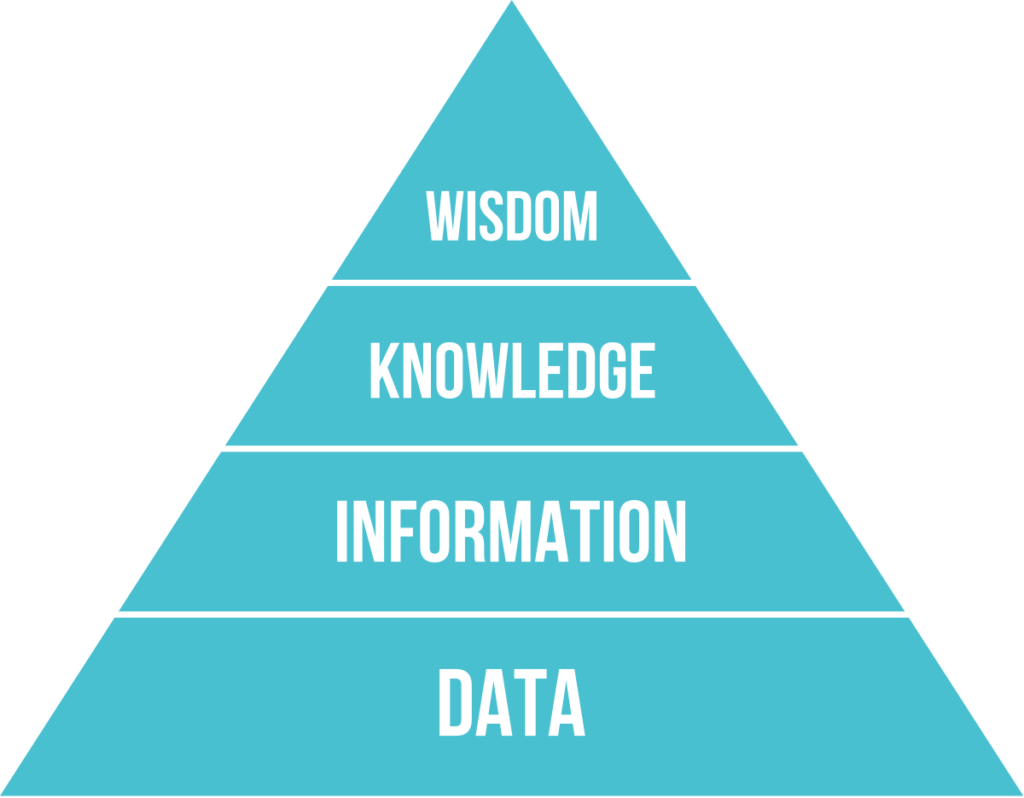
\includegraphics[scale=.3]{wkid.png}
\caption{Piramide DIKW}
\end{center}

\end{figure}

I \textbf{dati} sono costituiti da segni o simboli che rappresentano simboli o segnali che rimangono inutili fino  quando non sono messi in una qualche forma.  Possono essere \textit{universali} se sono prodotti da osservazioni, oppure \textit{soggettivi} costituite dalle osservazioni stesse. Possono essere costituiti da \textit{fatti}, cioè da osservazioni discrete, oggettive, non organizzate o elaborate che mancano di contesto interpretativo; da \textit{segnali}, cioè da stimoli sensoriali o letture di segnali attraverso sensi o sensori; o \textit{simboli}, cioè da insiemi di segni che rappresentano le percezioni di proprietà di oggetti, eventi dell'ambiente e che vengono registrati al fine della comunicazione.

Le \textbf{informazioni} sono dati dotati di significato e scopo, ottenute per descrizione e distinte dai dati per la oro utilità. Vengono inferite di dati rispondendo a specifiche domande o rendendoli utili a prendere decisioni.

La  \textbf{conoscenza} è definita come informazione elaborata, organizzata, o altrimenti applicata, messa in atto attraverso una commistione di esperienza sistematizzata, valori, informazioni contestuali, comprensione profonda e ben fondata. Fornisce un \textit{ambiente} e una struttura per la valutazione e l'acquisizione di nuove esperienza e informazioni nei singoli agenti, nei quali origina informazione e viene applicata a livello mentale, e nelle organizzazioni, spesso incorporata non solo attraverso documenti anche in senso esteso, e sistemi di memorizzazione, ma anche nelle procedure organizzative. Si possono definire inoltre diversi tipi i conoscenza:
\begin{itemize}
	\item \textbf{conoscenza elaborata} costituita dalla sintesi di più sorgenti di informazioni nel tempo, dalla comprensione, esperienza e apprendimento generati dall'organizzazione ed elaborazione dell'informazione. L'informazione è connessa attraverso relazioni di contesto, valori, esperienza e regole.
	
	\item \textbf{conoscenza procedurale} definita come conoscenza raggiunta attraverso un'esperienza pratica, quindi attraverso azioni e non attraverso delle descrizioni. In questo tipo di conoscenza si applicano dati e informazioni.
	
	\item \textbf{conoscenza proposizionale} descritta come strutturazione delle credenze e internalizzazione. In termini proposizionali la conoscenza può diventare a sua volta informazione, invece soggettivamente la conoscenza può essere costituita da un pensiero caratterizzato dalla credenza, che essa sia vera o meno, empirica o non emprica (logica, matematica, filosofia).
\end{itemize}

A questo punto possiamo dare una definizione di \textbf{Intelligenza Artificiale (AI)}:
\begin{center}
	"Disciplina che mira a studiare e comprendere i principi che rendono possibile un comportamento intelligente in sistemi artificiali."
\end{center}
quindi rendere vera l'equazione: ragionamento $\approx$ computazione. Un'ipotesi collegata è quella legata alla tesi di Church-Turing in cui nel quale il livello di astrazione del ragionamento equivale alla manipolazione dei simboli descritti come azioni/decisioni di un sistema spiegate in termini dei suoi input. Si mira a metodi per l progettazione di artefatti SW intelligenti, utili a scopi precisi.

Intelligenza dei sistemi è diversa da quella umana. Una comunità organizzata può esibire un comportamento intelligente, in quest'ambito si parla di \textbf{visione olistica} quando organizzazioni complesse, costituite da singole unità non particolarmente intelligenti, ma che nel loro complesso riescono a esibire un comportamento più intelligente.

L'AI come scienza mira a comprendere i principi del ragionamento secondo il metodo scientifico, attraverso il quale si dovrebbero creare e verificare teorie sulla soluzione algoritmica di problemi d'interesse supportate da implementazioni, attraverso anche la verifica sperimentale.

L'AI vista come disciplina ingegneristica, tesa a costruire tecnologie/sistemi che risolvano specifici problemi come quello di creare e testare sistemi software intelligenti basati su conoscenza.

\subsubsection{Progettazione di sistemi intelligenti basati su conoscenza}

Bisogna distinguere diverse fasi di computazione:
\begin{itemize}
\item \textbf{fase di progetto}, nella quale si gettano le basi del progetto in termini di requisiti
\item \textbf{offline}, nella quale elaboriamo le informazioni ricavate nella fase di progetto. In questa fase viene formalizzata la conoscenza che il sistema andrà a trattare, quindi si crea una base di conoscenza
\item \textbf{online}, fase nella quale si ottengono informazioni dalle osservazioni, prendendo decisioni usando la sua KB
\end{itemize}
La conoscenza del progettista è diversa dalla conoscenza nel KB del sistema, si possono distinguere due casi principali ed estremi: il sistema che andremo a creare sarà un \textbf{sistema specializzato} nel suo dominio/task ma inutile al di fuori di questo contesto, oppure il sistema che andremo a creare sarà un \textbf{sistema flessibile}, cioè che si adatta ai vari contesti. Inoltre, si possono distinguere diverse strategie di costruzione, partendo da una semplificazione del modello dell'ambiente/compito che però dovrà essere costruito attraverso sistemi di ragionamento complessi, oppure costruire un sistema semplice per contesti complessi.

Nell'AI è importante distinguere il \textbf{cosa} va calcolato dal \textbf{come} calcolarlo. La parte più difficile del procedimento è descrivere il dominio del problema, ovvero il cosa. Quindi bisogna far attenzione alla descrizione dei vari compiti. Uno \textit{schema generale} di risoluzione computazionale attraverso la formalizzazione parte dalla determinazione del cosa costituisca una soluzione, per poi rappresentare il problema in un linguaggio su cui il sistema possa ragionare, successivamente far calcolare al sistema un output e ala fine interpretarlo.

La conoscenza deve essere rappresentata attraverso un \textbf{linguaggio di rappresentazione} per formalizzare la conoscenza nelle macchine attraverso anche degli schemi di rappresentazione. Gli \textbf{schemi di rappresentazione} devono avere le seguenti proprietà:
\begin{itemize}
\item \textbf{ricchezza espressiva} sufficiente alla risoluzione del problema
\item \textbf{vicini} ai termini del problema
\item \textbf{efficienza} nell'elaborazione
\item \textbf{acquisibilità} da utenti, da dati e/o da esperienza pregressa
\end{itemize}
I linguaggi utilizzati sono pensati inizialmente per un solo obiettivo e man mano estesi per coprirne altri. Si possono utilizzare \textbf{linguaggi per l'apprendimento} estesi per ammettere maggiori capacità risolutive o di inferenza; \textbf{linguaggi espressivi} estesi per aggiungere capacità di inferenza e apprendimento; \textbf{linguaggi per la trattabilità} del calcolo resi in seguito più ricchi e naturali per agevolare l'acquisizione di conoscenza. 

La quantità di conoscenza dipende dal tipo di agente con il quale dobbiamo interagire. Un \textbf{agente umano} necessita di molta conoscenza per svolgere compiti anche molto semplici, mentre un \textbf{agente sw} necessita di poca conoscenza.

Per determinare le \textbf{soluzioni} del problema, il progettista deve spesso raffinare la specifica del problema. Vi possono essere diverse \textit{classi di soluzioni}:
\begin{itemize}
\item \textbf{soluzione ottimale}: che consiste in una soluzione che ha una \textbf{misura di qualità} ordinale o cardinale.
\item \textbf{soluzione soddisfacente}: che soddisfa le condizioni del problema sulla base di una certa soglia prefissata.
\item \textbf{soluzione approssimata}: in cui si misura quanto la qualità della soluzione trovata è lontana da quella ottimale.
\item \textbf{soluzione probabile}: soluzione che ha un certo grado di certezza, considerando anche un tasso di errore per indicare falsi positivi e falsi negativi.
\end{itemize}

Nella \textbf{rappresentazione} di un problema, si ha un sistema i simboli volti ad acquisire e rappresentare la conoscenza su un dominio e come utilizzarla per rispondere a domande e/o risolvere problemi.  L'ipotesi di Newell $\&$ Simon definisce un sistema di simboli fisici come un sistema che ha gli strumenti necessari e sufficienti per compiere delle azioni intelligenti. Un sistema intelligente manipola simboli per ragionare: simboli che si riferiscono ai vari oggetti del mondo esterno e simboli interni che rimandano a concetti utili. Un sistemi di simboli serve a modellare il mondo, per rappresentare ciò che deve essere considerato vero nel mondo o della sua dinamica. Quindi attraverso la modellazione del mondo in simboli si crea un'astrazione di esso molto utile, che può essere soddisfatta a diversi livelli dettati dalla profondità in cui si vuole scendere in dettaglio. Un sistema può avere anche più modelli di astrazione, anche in contraddizione tra loro, che vengono giudicati in base all'utilità.

Si parla di \textbf{singolo} livello di astrazione quando si descrive il modello del mondo in base a un livello più alto, comprensibile anche dall'uomo e molto generico, oppure a un livello più basso, con descrizioni più accurate e predittive, comprensive di dettagli essenziali per la risoluzione del problema. Più basso è il livello, più difficile è il ragionamento e si devono compiere più passi e più piani d'azione da scegliere.

Si hanno modelli a pi livelli d'astrazione quando ad esempio di creano progetti multidisciplinari, i quali possono condividere alcune parti.

\subsubsection{Progetto - Dimensione della complessità}

Il sistema ha diverse \textbf{dimensioni} della sua complessità nella progettazione da combinare anche se studiate separatamente, e che definiscono uno spazio di progettazione di sistemi intelligenti, diversi a seconda dei loro valori. Queste dimensioni forniscono una \textit{decomposizione sommaria} dello spazio di progettazione, anche se devono essere aggiunte altre scelte. Ogni agente ha una sua \textbf{complessità} variabile.

Vi sono diverse dimensioni di complessità:
\begin{itemize}
\item Modularità
\item Schema di rappresentazione
\item Incertezza sull'osservazione
\item Incertezza sull'effetto
\item Preferenze
\item Apprendimento
\item Limiti Risorse Computazionali
\item Orizzonte
\item Numero di Attori
\end{itemize}

La \textbf{modularità} è il grado di decomposizione di un sistema in moduli integrati a prendere in considerazione separatamente. Serve a dominare la complessità ed è tipicamente espressa come decomposizione gerarchica, ovvero ogni modulo organizzato in sotto-moduli a loro volta organizzati gerarchicamente fino al livello delle operazioni primitive attraverso l'utilizzo dell'astrazione procedurale e l'OOP. Vi sono diverse strutture possibili: \textbf{piatta} se non vi è nessuna struttura organizzativa, \textbf{modulare} se il sistema è decomposto in moduli interagenti considerabili separatamente, \textbf{gerarchica} se vi è un sistema modulare dove i moduli possono essere decomposti in sotto moduli interagenti, a loro volta decomponibili gerarchicamente.

Nella struttura piatta e modulare vi è un singolo livello di astrazione, mentre nella struttura gerarchica sono presenti più processi, più basso è il livello nella gerarchia e pi basso sarà il livello di astrazione. Nella struttura gerarchica, solamente in una fase iniziale si potrebbe ignorare l'aspetto gerarchico per concentrarsi anche sulle altre dimensioni della complessità, utile soprattutto per problemi modesti.

Lo \textbf{schema di rappresentazione} riguarda la descrizione del mondo in stati distinti che hanno un impatto sul comportamento del sistema, fattorizzabile in stato interno e stato dell'ambiente, nel quale il caso più semplice consiste in un sistema che ragiona esplicitamente in termini di stati identificati individualmente. Quando lo stato è descrivibile in termini di caratteristiche con un valore per ogni stato. Una proposizione è una caratteristica boolean che può assumere valori di vero/falso. Nella descrizione di mondi complessi le caratteristiche dipendono dalle relazioni e dagli individui: una relazione su un singolo individuo è una \textbf{proprietà} e si può definire una caratteristica per ogni possibile relazione tra gli individui. In alcuni casi può essere conveniente trattare descrizioni relazionali in termini di individui e relazioni invece di caratteristiche e proposizioni. Infatti ragionando su relazioni e individui, si possono considerare intere classi di individui senza enumerarne caratteristiche o proposizioni o addirittura i numerosi stati.

Alcune volte si progetta tenendo conto dell'\textbf{incertezza} insita nel dominio considerato in termini di percezione, osservazione, effetti delle decisioni e azioni. A volte è possibile \textbf{l'osservazione diretta} dello stato del mondo, altre volte può accadere che la percezione dello stato sia \textbf{difettosa o parziale/indiretta}, al più si può ottenere una distribuzione di probabilità sull'insieme degli stati possibili su quanto si osserva. In questi casi si parla di \textbf{incertezza sulla percezione} che riguarda la possibilità di terminare lo stato del mondo attraverso osservazioni. Se lo stato è \textbf{pienamente osservabile} si può conoscere dalle osservazioni, altrimenti se è osservato indirettamente si parla di \textbf{stato parzialmente osservabile}.

A volte è possibile conoscere l'effetto delle decisioni/azioni, quindi dato uno stato e un'azione/decisione, si può predire precisamente lo stato risultante dall'applicazione dell'azione/decisione. A volte però è difficile fare tali previsioni, al più si può avere una distribuzione di probabilità sugli effetti possibili. L'\textbf{incertezza sugli effetti} prevede che la loro dinamica possa essere \textit{deterministica}, quindi lo stato risultante è determinato dall'azione e dallo stato precedente, mentre è \textbf{aleatorio} quando ogni stato risultante ha una determinata probabilità di poter essere ottenuto e ha senso solo se il mondo è completamente osservabile.

Gli agenti sono spesso \textbf{utilitaristici}, ovvero la scelta di un'azione è dettata da risuòtati attesi più desiderabili e hanno finalità semplici o preferenze complesse (stato da raggiungere o proposizione da avverare). Le \textbf{preferenze} si caratterizzano come:
\begin{itemize}
\item \textbf{finalità}, da raggiungere in uno stato finale o di conservazione in ogni stato visitato
\item \textbf{preferenze complesse}, ovvero compromessi sul vantaggio derivate dei vari risultati, eventualmente anche in momenti diversi. Si possono distinguere:
	\begin{itemize}
		\item \textbf{preferenza ordinale}: conta solo l'ordine
		\item \textbf{preferenza cardinale}: conta anche la grandezza del valore
	\end{itemize}
\end{itemize}

Non sempre il progettista dispone di un buon modello del sistema e del suo ambiente, si devono usare dati da esperienze passate e altre sorgenti di conoscenza per migliorare il modello e prendere migliori decisioni. La dimensione dell'\textbf{apprendimento} determina se la conoscenza sia data o vada appresa dai dati o da esperienza pregressa. Quindi apprendere significa trovare il modello migliore che si adatti ai dati e  in questa situazione si potrebbe verificare un caso semplice in cui bisogna regolare un insieme fisso di parametri o nel caso più difficile scegliere preliminarmente la migliore rappresentazione. Vi sono però anche delle problematiche, quali l'utilizzo di conoscenza i fondo, selezione dei dati da raccogliere, rappresentazione dei dati e dei modelli, selezione dei learning bias appropriati.

I \textbf{limiti sulle risorse computazionali} spesso impediscono di prendere le migliori decisioni sulle azioni da svolgere. Non sarà possibile trovare la migliore decisione in modo sufficientemente rapido date le limitazioni sulla memoria, oppure bisogna fare dei compromessi sulla qualità della soluzione da cercare. Tale dimensione determina se il sistema ragiona per prendere la migliore decisione senza tenere conto dei limiti (\textbf{razionalità perfetta})) o tenendo conto dei limitati (\textbf{razionalità limitata}). I limiti riguardano il tempo, la memoria e la precisione approssimata. Un \textbf{algoritmo anytime} produce soluzioni che migliorano nel tempo, produce sempre la migliore soluzione corrente, si assicura che la qualità non decresca conservando la migliore soluzione trovata da restituire su richiesta, mentre vi è un costo per l'attesa perchè a volte è meglio agire/decidere subito anzichè di aspettare una soluzione probabilmente migliore. In caso di razionalità limitata si deve decidere se aspettare o pensare un po' di più in quanto è difficile giudicare la politica migliore, anche il tempo speso per decidere è da sottrarre a quello di ricerca della soluzione e motva il cosiddetto ragionamento approssimato.

\textbf{L'orizzonte} misura quanto lontano sia prevista la pianificazione del lavoro, ossia quanto in avanti ci si spinga a considerare le conseguenze delle azioni. In tale dimensione si possono avere sistemi/agenti SW:
\begin{itemize}
\item \textbf{senza pianificazione}: che considerano il futuro quando prendono decisioni sulle azioni, quindi non viene coinvolto il fattore-tempo
\item \textbf{a orizzonte finito}: interessano solo un numero prefissato di passi
\item \textbf{a orizzonte indefinito}: si considera un numero di passi finito, ma non predeterminato
\item \textbf{a orizzonte infinito}: sempre attivo
\end{itemize}

Vi sono delle difficoltà aggiuntive degli ambienti con altri agenti/sistemi, occorre ragionare sugli altri agenti secondo strategie in quanto potrebbero cercare di confondere e manipolare o potrebbero cooperare, anche quando si cooperi e vi sia un fine comune, il problema della coordinazione e della comunicazione rende il ragionamento multi-agente pi complesso. Dal punto di vista del singolo agente, la dimensione del numero di agenti prevede:
\begin{itemize}
\item un \textbf{ragionamento da agente singolo}, cioè si assume che gli altri siano parte dell'ambiente, utile se non ci sono altri agenti o se gli altri non cambierano il comportamento in base alle sue azioni
\item \textbf{ragionamento multi-agente}, in cui si prende in considerazione il ragionamento degli altri agenti nel caso di agenti intelligenti i cui fini/preferenze dipendano, in parte, da quello che si fa se l'agente può comunicare con gli altri, più difficile se gli agenti possono agire simultaneamente o se l'ambiente è solo parzialmente osservabile.
\end{itemize}

\subsubsection{Agenti e sistemi intelligenti}

Gli \textbf{agenti intelligenti} sono elementi la cui percezione/ragionamento/azione dipende dall'ambiente in cui sono immersi, definito anche come mondo. Il loro comportamento dipende anche in base a una conoscenza pregressa su agente e ambiente, sulla storia dell'interazione con l'ambiente attraverso stimoli ed esperienza passata, dagli obiettivi da raggiungere o da preferenze sugli stati del mondo e dalle abilità, cioè azioni primitive di cui è capace.

All'interno dell'agente quindi si memorizza lo stato interno delle credenze, cioè s rappresentano le cose che si ritengono vere circa l'ambiente, cosa si è imparato, gli obiettivi intermedi presenti e futuri, gli aggiornamenti in base agli stimoli e ciò che serve a prendere decisioni. A un dato livello di astrazione vi sono 4 compiti:
\begin{itemize}
\item \textbf{Modellazione dell'ambiente}: come ottenere le info, quali risposte siano ammesse alle domande e quali info siano necessarie per rispondere
\item \textbf{Ragionamento sulle evidenze} (o percezioni): determinare com'è fatto il dominio, dove sono disponibili le info.
\item \textbf{Azione}: dato un modello del mondo e uno scopo, si determina cosa va fatto per raggiungerlo ed eventualmente si consultano una o più basi di conoscenza per estrarre informazioni.
\item \textbf{Apprendimento dall'esperienza passata}: imparare le caratteristiche dell'ambiente
\end{itemize}
Un'interazione nello svolgimento di tali compiti comporta uno studio organico.

Un KBS gestisce nel tempo un modello del mondo più o meno complesso, considerando due casi limite del sistema: il ragionamento sul modello ignorando le percezioni e il ragionamento alle percezioni. In genere queste capacità sono combinate. Un \textbf{sistema basato sulla conoscenza} (KBS) consiste in un modello del dominio per risolvere problemi, attraverso anche la \textbf{conoscenza} costituita da informazioni sul dominio usabili per decidere/agire su di esso, ma costituita anche da credenze. Queste informazioni possono essere costituite da informazioni generali e persistenti considerate come vere a lungo termine e credenze più transienti destinate a essere cambiate più frequentemente.

La KB è costituita da due momenti principali distinti:
\begin{itemize}
\item un processo \textbf{Online} che comprende tutte quelle operazioni di ragionamento tipiche del KB, osservazioni e abilità per prendere decisioni e aggiornare la KB stessa. 
\item un processo ofline, nel quale utilizza la conoscenza pregressa ed esperienze passate, anche in forma di dati, e si costruisce la KB. Però servono molti dati e conoscenza generale,, soprattutto a livello statistico.
\end{itemize}

In una fase di progetto e offline è fondamentale rappresentare il dominio del problema da risolvere o del compito da svolgere, descrivendo in che cosa consiste il domnio e da quali legami siano correlate. Inoltre devono essere specificati i simboli usati dal sistema con la rappresentazione esplicita in termini di stati completamente osservabili. Il KB viene quindi costruito combinando conoscenza di esperti e dati.

Nella modalità online invece si rendono disponibili informazioni sulla particolare situazione corrente e si può ragionare o agire anche in base alle osservazioni derivanti da sensori, utenti o altri agenti. Si coinvolgono gli utenti che hanno esperienza necessaria a fornire info su situazioni individuali, non devono essere quindi degli esperti del dominio e non conoscono cosa sia effettivamente al sistema; i sensori che forniscono informazioni sull'ambiente e possono essere distinti sia in sensori attivi, quando vengono controllati o interrogati, e sensori passivi quando forniscono solo feedback; infine vi sono le sorgenti esterne di conoscenza come u sito web o un database cui chiedere domande su un dominio limitato.

\subsubsection{Applicazioni prototipiche}

Sono particolari domini applicativi che possono essere riassunti nel caso della smart house come robot per la consegna, assistente per la diagnostica, sistemi di tutoring o assistente agli acquisti. Un \textbf{inforobot} è un robot che interagisce con un ambiente informativo anzichè fisico. I suoi compiti consistono nell'estrarre informazioni da una rete di sorgenti informative, determinare quale informazione serva per una query e individuare le sorgenti informative, trovare le informazioni necessarie e presentarle in modo utile per l'utente. In input riceve conoscenza pregressa, esperienza passata, le finalità, le osservazioni e le abilità e come output da un info utile alla comprensione da parte dell'utente. Un inforobot deve essere capace di derivare informazione implicita nella base di conoscenza, cercare informazione rilevante in una varietà di basi di conoscenza, trovare buone rappresentazioni della conoscenza, spiegare come sia stata derivata una risposta o perchè alcune informazioni non erano più disponibili.
\newpage
\subsection{2 - Spazi di stati e Ricerca di soluzioni}
Questa sezione fa riferimento al capitolo 3 del libro.

Nel caso più semplice il sistema ragiona su \textbf{un modello} del mondo fatto di stati, in assenza \textbf{di incertezza}, con \textbf{un obiettivo} da raggiungere. Si rappresenta il mondo con una rappresentazione non gerarchica, ovvero una rappresentazione \textbf{piatta}, e si pone come obiettivo quello di trovare la sequenza di passi nello spazio degli stati, partendo dallo stato corrente fino ad un obiettivo. Quindi vi è necessità di astrarre il dominio del problema attraverso la ricerca di un percorso in un grafo orientato, partendo da un nodo di partenza fino a un nodo finale. Vi sono molti algoritmi disponibili che risolvono questo problema, i quali effettuano una computazione all'interno del sistema.

Si definisce \textbf{navigatore} quando si ricerca il miglior percorso in base alla lunghezza (più corto), al tempo di percorrenza (velocità) e il costo (costo minimo). In questo problema si ha anche lo stato che indica la localizzazione corrente dell'oggetto, compresa la velocità e la direzione. Il sistema costruisce una serie di soluzioni parziali.
\newpage
\section{Libro}

\subsection{Capitolo 1 - Intelligenza artificiale e agenti}

\begin{center}
"La storia dell'IA è una storia di fantasie, possibilità, dimostrazioni e promesse. Da quando Omero scrisse di "treppiedi" meccanici che aspettavano gli dei a cena, gli assistenti meccanici immaginari hanno fatto parte della nostra cultura. Tuttavia, solo nell'ultimo mezzo secolo noi, la comunità dell'IA, siamo stati in grado di costruire macchine sperimentali che testano ipotesi sui meccanismi del pensiero e del comportamento intelligente e quindi dimostrano meccanismi che in precedenza esistevano solo come possibilità teoriche."
Bruce Buchanan
\end{center}

Questo libro parla dell'intelligenza artificiale, un campo costruito su secoli di pensiero, disciplina riconosciuta da oltre 60 anni. Come sottolinea Buchanan nella citazione sopra, ora abbiamo gli strumenti per testare ipotesi sulla natura del pensiero stesso, così come per risolvere compiti pratici. I profondi problemi scientifici e ingegneristici sono già stati risolti e molti altri aspettano di essere risolti. Molte applicazioni pratiche sono attualmente implementate e il potenziale esiste per un numero quasi illimitato di applicazioni future. In questo libro presentiamo i principi che stanno alla base degli agenti computazionali intelligenti. Questi principi possono aiutarti a comprendere il lavoro attuale e futuro nell'IA e prepararti a contribuire tu stesso alla disciplina.

\subsubsection{Che cos'è l'intelligenza artificiale?}

\textbf{L'intelligenza artificiale}, o AI, è il campo che studia la sintesi e l'analisi di agenti computazionali che agiscono in modo intelligente. Un \textbf{agente} è qualcosa che agisce in un ambiente; fa qualcosa. Siamo interessati a ciò che fa un agente; cioè come agisce . Giudichiamo un agente dalle sue azioni. Un agente agisce in modo intelligente quando:
\begin{itemize}
\item ciò che fa è appropriato alle sue circostanze e ai suoi obiettivi, tenendo conto delle conseguenze a breve ea lungo termine delle sue azioni
\item è flessibile al cambiamento degli ambienti e al cambiamento degli obiettivi
\item impara dall'esperienza
\item fa scelte appropriate date le sue limitazioni percettive e computazionali
\end{itemize}
\textbf{Un agente computazionale} è un agente le cui decisioni sulle sue azioni possono essere spiegate in termini di calcolo. Cioè, la decisione può essere scomposta in operazioni primitive che possono essere implementate in un dispositivo fisico. Questo calcolo può assumere molte forme. Tutti gli agenti sono limitati. Nessun agente è onnisciente o onnipotente. Gli agenti possono osservare tutto ciò che riguarda il mondo solo in domini molto specializzati, dove "il mondo" è molto limitato. Gli agenti hanno memoria limitata. Gli agenti nel mondo reale non hanno tempo illimitato per agire.

\textbf{L'obiettivo scientifico} centrale dell'IA è comprendere i principi che rendono possibile un comportamento intelligente nei sistemi naturali o artificiali. Questo è fatto da:
\begin{itemize}
\item l' analisi degli agenti naturali e artificiali
\item formulare e testare ipotesi su ciò che serve per costruire agenti intelligenti 
\item progettare, costruire e sperimentare sistemi computazionali che svolgono compiti comunemente considerati come richiedenti intelligenza.
\end{itemize}

Nell'ambito della scienza, i ricercatori costruiscono sistemi empirici per testare ipotesi o per esplorare lo spazio di possibili progetti. Questi sono abbastanza distinti dalle applicazioni create per essere utili per un dominio di applicazioni. La definizione non è solo per il pensiero intelligente. Ci interessa pensare in modo intelligente solo nella misura in cui porta a un comportamento più intelligente. Il ruolo del pensiero è di influenzare l'azione. L'obiettivo ingegneristico centrale dell'IA è la progettazione e la sintesi di artefatti utili e intelligenti. In realtà vogliamo creare agenti che agiscano in modo intelligente. Tali agenti sono utili in molte applicazioni.

\subsubsection{Agenti Situati in Ammbienti}
L'IA riguarda il ragionamento pratico: ragionare per fare qualcosa. Un accoppiamento di percezione, ragionamento e azione comprende un agente. Un agente agisce in un ambiente. L'ambiente di un agente può anche includere altri agenti. Un agente insieme al suo ambiente è chiamato mondo.

Un agente potrebbe essere, ad esempio, un accoppiamento di un motore computazionale con sensori e attuatori fisici, chiamato robot, in cui l'ambiente è un ambiente fisico. Potrebbe essere l'accoppiamento di un computer che dà consigli, un sistema esperto, con un essere umano che fornisce informazioni percettive e svolge il compito. Un agente potrebbe essere un programma che agisce in un ambiente puramente computazionale, un agente software. In qualsiasi momento, ciò che fa un agente dipende da:
\begin{itemize}
\item \textbf{conoscenza preliminare} dell'agente e dell'ambiente
\item \textbf{storia} di interazione con l'ambiente, di cui è composto:
\begin{itemize}
\item \textbf{stimoli} ricevuti dall'ambiente attuale, che possono includere osservazioni sull'ambiente, nonché azioni che l'ambiente impone all'agente 
\item \textbf{esperienze passate} di azioni e stimoli precedenti, o altri dati, da cui può imparare
\end{itemize}
\item \textbf{obiettivi} che deve cercare di raggiungere o preferenze rispetto agli stati del mondo
\item \textbf{abilità} le azioni primitive che l'agente è in grado di compiere.
\end{itemize}

All'interno della scatola nera, un agente ha \textbf{uno stato di convinzione} interna che può codificare le convinzioni sul suo ambiente, su ciò che ha imparato, su ciò che sta cercando di fare e su ciò che intende fare. Un agente aggiorna questo stato interno in base agli stimoli. Usa lo stato di convinzione e gli stimoli per decidere le sue azioni. Gran parte di questo libro parla di cosa c'è dentro questa scatola nera. Questa è una visione onnicomprensiva di agenti intelligenti che variano in complessità da un semplice termostato, a un sistema di consulenza diagnostica le cui percezioni e azioni sono mediate da esseri umani, a una squadra di robot mobili, alla società stessa. \textbf{Gli agenti intenzionali} hanno preferenze o obiettivi. Preferiscono alcuni stati del mondo ad altri stati e agiscono per cercare di raggiungere gli stati che preferiscono di più. Gli agenti non finalizzati sono raggruppati insieme e chiamati natura . Il fatto che un agente sia intenzionale o meno è un presupposto di modellazione che può essere appropriato o meno. Ad esempio, per alcune applicazioni può essere opportuno modellare un cane come intenzionale, e per altre può essere sufficiente modellare un cane come non intenzionale. Se un agente non ha preferenze, per definizione non gli importa in quale stato mondiale finisce, e quindi non gli importa cosa fa. Il motivo per progettare un agente è instillare le preferenze in esso: farlo preferire alcuni stati del mondo e cercare di raggiungerli. Un agente non deve conoscere le sue preferenze in modo esplicito. Ad esempio, un termostato è un agente che rileva il mondo e accende o spegne un riscaldatore. Ci sono preferenze incorporate nel termostato, come mantenere gli occupanti di una stanza a una temperatura piacevole, anche se il termostato probabilmente non sa che queste sono le sue preferenze. Le preferenze di un agente sono spesso le preferenze del progettista dell'agente, ma a volte un agente può acquisire obiettivi e preferenze in fase di esecuzione.

\subsubsection{Agenti di progettazione}

Gli agenti artificiali sono progettati per compiti particolari. I ricercatori non sono ancora arrivati alla fase di progettazione di un agente per il compito di sopravvivere e riprodursi in un ambiente naturale. Nel decidere cosa farà un agente, ci sono tre aspetti del calcolo che devono essere distinti: (1) il calcolo che entra nella progettazione dell'agente, (2) il calcolo che l'agente può fare prima di osservare il mondo e ha bisogno agire e (3) il calcolo che viene eseguito dall'agente mentre agisce. \textbf{Il calcolo del tempo di progettazione} è il calcolo che viene eseguito per progettare l'agente. Viene eseguito dal progettista dell'agente, non dall'agente stesso. \textbf{Il calcolo offline} è il calcolo eseguito dall'agente prima che debba agire. Può includere la compilazione e l'apprendimento. Offline, un agente può acquisire conoscenze e dati di base e compilarli in una forma utilizzabile chiamata knowledge base. Le conoscenze di base possono essere fornite in fase di progettazione o offline. \textbf{Il calcolo online} è il calcolo eseguito dall'agente tra l'osservazione dell'ambiente e l'azione nell'ambiente. Un'informazione ottenuta online è chiamata osservazione . Un agente in genere deve utilizzare la sua base di conoscenze, le sue convinzioni e le sue osservazioni per determinare cosa fare dopo.

È importante distinguere tra la conoscenza nella mente del progettista e la conoscenza nella mente dell'agente. A un estremo c'è un agente altamente specializzato che funziona bene nell'ambiente per il quale è stato progettato, ma è indifeso al di fuori di questa nicchia. Il progettista potrebbe aver svolto un lavoro considerevole nella creazione dell'agente, ma l'agente potrebbe non aver bisogno di fare molto per funzionare bene. Un esempio è un termostato. Potrebbe essere difficile progettare un termostato in modo che si accenda e si spenga esattamente alle temperature giuste, ma il termostato stesso non deve fare molti calcoli. Un altro esempio è un robot per la verniciatura di automobili che dipinge sempre le stesse parti in una fabbrica di automobili. Potrebbe essere necessario molto tempo di progettazione o calcolo offline per farlo funzionare perfettamente, ma il robot di verniciatura può dipingere parti con pochi calcoli online; intuisce che c'è una parte in posizione, ma poi esegue le sue azioni predefinite. Questi agenti molto specializzati non si adattano bene ad ambienti diversi oa obiettivi mutevoli. Il robot di verniciatura non si accorgerebbe se fosse presente un tipo diverso di parte e, anche se lo facesse, non saprebbe cosa farne. Dovrebbe essere ridisegnato o riprogrammato per verniciare parti diverse o per trasformarlo in una levigatrice o in una lavatrice per cani. All'altro estremo c'è un agente molto flessibile che può sopravvivere in ambienti arbitrari e accettare nuove attività in fase di esecuzione. Semplici agenti biologici come gli insetti possono adattarsi a complessi ambienti mutevoli, ma non possono svolgere compiti arbitrari. Progettare un agente in grado di adattarsi ad ambienti complessi e obiettivi mutevoli è una sfida importante. L'agente saprà molto di più sui particolari di una situazione rispetto al progettista. Anche la biologia non ha prodotto molti di questi agenti. Gli esseri umani possono essere l'unico esempio esistente, ma anche gli esseri umani hanno bisogno di tempo per adattarsi a nuovi ambienti.

Anche se l'agente flessibile è il nostro sogno finale, i ricercatori devono raggiungere questo obiettivo attraverso obiettivi più banali. Piuttosto che costruire un agente universale, che può adattarsi a qualsiasi ambiente e risolvere qualsiasi compito, hanno costruito agenti particolari per particolari nicchie ambientali. Il progettista può sfruttare la struttura della nicchia particolare e l'agente non deve ragionare su altre possibilità. Due grandi strategie sono state perseguite nello sviluppo degli agenti:
\begin{itemize}
\item Il primo è semplificare gli ambienti e costruire complessi sistemi di ragionamento per questi ambienti semplici.
\item La seconda strategia consiste nel costruire agenti semplici in ambienti naturali.
\end{itemize}

Uno dei vantaggi della semplificazione degli ambienti è che può permetterci di provare le proprietà degli agenti o di ottimizzare gli agenti per situazioni particolari. La verifica delle proprietà o l'ottimizzazione in genere richiede un modello dell'agente e del relativo ambiente. L'agente può ragionare un po' o molto, ma un osservatore o un progettista dell'agente può essere in grado di ragionare sull'agente e sull'ambiente. Ad esempio, il progettista potrebbe essere in grado di dimostrare se l'agente può raggiungere un obiettivo, se può evitare di entrare in situazioni che potrebbero essere dannose per l'agente (sicurezza), se rimarrà bloccato da qualche parte (vivacità) o se lo farà alla fine si occuperà di ciascuna delle cose che dovrebbe fare (equità).

Un modo in cui le rappresentazioni dell'IA differiscono dai programmi per computer nei linguaggi tradizionali è che una rappresentazione dell'IA in genere specifica cosa deve essere calcolato, non come deve essere calcolato. Potremmo specificare che l'agente dovrebbe trovare la malattia più probabile che ha un paziente, o specificare che un robot dovrebbe prendere il caffè, ma non dare istruzioni dettagliate su come fare queste cose. Gran parte del ragionamento basato sull'IA implica la ricerca nello spazio delle possibilità per determinare come completare un'attività.


\begin{figure}[h!]
\begin{center}
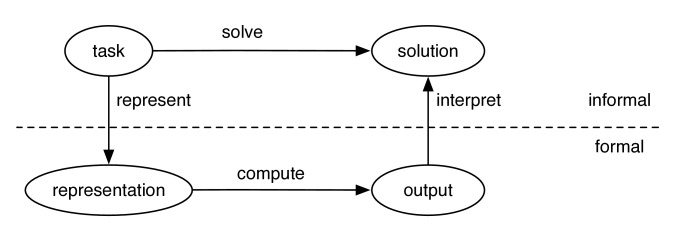
\includegraphics[scale=.65]{ruoloAgenti.png}
\caption{Ciclo agente}
\end{center}
\end{figure}
Per risolvere un compito, il progettista di un sistema deve:
\begin{itemize}
\item determinare cosa costituisce una soluzione
\item rappresentare l'attività in un modo in cui un computer può ragionare
\item utilizzare il computer per calcolare un output, ovvero le risposte presentate a un utente o le azioni da eseguire nell'ambiente
\item interpretare l'output come una soluzione al compito.
\end{itemize}

\textbf{La conoscenza} è l'informazione su un dominio che può essere utilizzata per risolvere compiti in quel dominio. Per risolvere molti compiti è necessaria molta conoscenza e questa conoscenza deve essere rappresentata nel computer. Come parte della progettazione di un programma per risolvere compiti, dobbiamo definire come sarà rappresentata la conoscenza. Un \textbf{linguaggio di rappresentazione} viene utilizzato per esprimere la conoscenza utilizzata in un agente. \textbf{Una rappresentazione} di alcune conoscenze sono le particolari strutture di dati utilizzate per codificare la conoscenza in modo che possa essere ragionata. \textbf{Una base di conoscenza} è la rappresentazione di tutta la conoscenza memorizzata da un agente.
Un buon linguaggio di rappresentazione è un compromesso tra molti obiettivi concorrenti. Una rappresentazione dovrebbe essere:
\begin{itemize}
\item abbastanza ricco da esprimere le conoscenze necessarie per risolvere il compito
\item il più vicino possibile a una specificazione naturale del compito; dovrebbe essere compatto, naturale e manutenibile. Dovrebbe essere facile vedere la relazione tra la rappresentazione e il dominio rappresentato, in modo che sia facile determinare se la conoscenza rappresentata è corretta. Una piccola modifica nell'attività dovrebbe comportare una piccola modifica nella rappresentazione dell'attività
\item suscettibile di calcolo efficiente, o trattabile , il che significa che l'agente può agire abbastanza rapidamente. Per garantire ciò, le rappresentazioni sfruttano le caratteristiche dell'attività per il guadagno computazionale e compensano l'accuratezza e il tempo di calcolo
\item in grado di essere acquisito da persone, dati ed esperienze passate.
\end{itemize}

Data una descrizione informale di un'attività, prima ancora di considerare un computer, un progettista agente dovrebbe determinare cosa costituirebbe una soluzione. Questa domanda sorge non solo nell'IA, ma in qualsiasi progettazione di software. Gran parte dell'ingegneria del software implica il perfezionamento delle specifiche dell'attività. Le attività in genere non sono ben specificate. Non solo di solito c'è molto non specificato, ma anche le parti non specificate non possono essere compilate arbitrariamente. Data un'attività ben definita, il problema successivo è se è importante se la risposta restituita è errata o incompleta. Esistono quattro classi comuni di soluzioni:
\begin{itemize}
\item Una \textbf{soluzione ottimale} per un'attività è quella che è la soluzione migliore in base a una certa misura della qualità della soluzione.
\item Spesso un agente non ha bisogno della soluzione migliore per un'attività, ma ha solo bisogno di una soluzione. \textbf{Una soluzione soddisfacente} è quella che è abbastanza buona secondo una descrizione di quali soluzioni sono adeguate.
\item Uno dei vantaggi di una misura cardinale del successo è che consente approssimazioni. Una \textbf{soluzione approssimativamente ottimale} è quella la cui misura della qualità è vicina al meglio che potrebbe essere teoricamente ottenuto. In genere, gli agenti non necessitano di soluzioni ottimali per le attività; devono solo avvicinarsi abbastanza. Per alcune attività, dal punto di vista computazionale è molto più facile ottenere una soluzione approssimativamente ottimale che ottenere una soluzione ottimale. Tuttavia, per altre attività, è altrettanto difficile trovare una soluzione approssimativamente ottimale che sia garantita entro alcuni limiti dell'ottimo quanto trovare una soluzione ottimale.

\item \textbf{Una soluzione probabile} è quella che, anche se potrebbe non essere effettivamente una soluzione per l'attività, è probabile che sia una soluzione. Questo è un modo per approssimare, in modo preciso, una soluzione soddisfacente. Spesso si vuole distinguere il tasso di errore falso positivo (la proporzione di risposte fornite dal computer che non sono corrette) dal tasso di errore falso negativo (la proporzione di quelle risposte non fornite dal computer che sono effettivamente corrette). Alcune applicazioni sono molto più tolleranti di uno di questi tipi di errori rispetto all'altro.
\end{itemize}

Una volta che hai alcuni requisiti sulla natura di \textbf{una soluzione}, devi rappresentare l'attività in modo che un computer possa risolverla. I computer e le menti umane sono esempi di sistemi di simboli fisici. \textbf{Un simbolo} è un modello significativo che può essere manipolato. Esempi di simboli sono parole scritte, frasi, gesti, segni su carta o sequenze di bit. Un sistema di simboli crea, copia, modifica e distrugge i simboli. In sostanza, un simbolo è uno dei modelli manipolati come unità da un sistema di simboli. Viene usato il termine fisico, perché i simboli in un sistema di simboli fisici sono oggetti fisici che fanno parte del mondo reale, anche se possono essere interni ai computer e al cervello. Potrebbero anche aver bisogno di influenzare fisicamente l'azione o il controllo motorio. Gran parte dell'IA si basa sull'ipotesi del sistema di simboli fisici di Newell e Simon: Un sistema di simboli fisici ha i mezzi necessari e sufficienti per un'azione intelligente generale.

Significa che qualsiasi agente intelligente è necessariamente un sistema di simboli fisici. Significa anche che un sistema di simboli fisici è tutto ciò che è necessario per un'azione intelligente; non è richiesta alcuna magia o un fenomeno quantistico ancora da scoprire. Non implica che un sistema di simboli fisici non abbia bisogno di un corpo per percepire e agire nel mondo. Si discute se le variabili nascoste, a cui non è stato assegnato un significato, ma sono utili, possano essere considerate come simboli. L'ipotesi del sistema dei simboli fisici è un'ipotesi empirica che, come altre ipotesi scientifiche, deve essere giudicata da quanto bene si adatta alle prove e da quali ipotesi alternative esistono. In effetti, potrebbe essere falso.

Un agente intelligente può essere visto come un manipolatore di simboli per produrre azioni. Molti di questi simboli sono usati per riferirsi a cose nel mondo. Altri simboli possono essere concetti utili che possono avere o meno un significato esterno. Ancora altri simboli possono riferirsi a stati interni dell'agente. Un agente può utilizzare un sistema di simboli fisici per modellare il mondo. \textbf{Un modello} di mondo è una rappresentazione delle convinzioni di un agente su ciò che è vero nel mondo o su come il mondo cambia. Il mondo non deve essere modellato al livello più dettagliato per essere utile. Tutti \textbf{i modelli} sono astrazioni ; rappresentano solo una parte del mondo e tralasciano molti dettagli. Un agente può avere un modello molto semplicistico del mondo, oppure può avere un modello molto dettagliato del mondo. \textbf{Il livello di astrazione} fornisce un ordinamento parziale dell'astrazione. Un'astrazione di livello inferiore include più dettagli rispetto a un'astrazione di livello superiore. Un agente può avere modelli del mondo multipli, anche contraddittori. I modelli vengono giudicati non in base alla loro correttezza, ma in base alla loro utilità.

La scelta di un livello di astrazione appropriato è difficile per i seguenti motivi:
\begin{itemize}
\item Una descrizione di alto livello è più facile da specificare e comprendere per un essere umano.
\item Una descrizione di basso livello può essere più accurata e più predittiva. Spesso le descrizioni di alto livello sottraggono dettagli che possono essere importanti per risolvere effettivamente il compito.
\item Più basso è il livello, più difficile è ragionare. Questo perché una soluzione a un livello di dettaglio inferiore comporta più passaggi ed esistono molte più possibili linee di azione tra cui scegliere.
\item Un agente potrebbe non conoscere le informazioni necessarie per una descrizione di basso livello.
\end{itemize}

Spesso è una buona idea modellare un ambiente a più livelli di astrazione. Due tipi di livelli di astrazione molto comuni sono:
\begin{itemize}
\item \textbf{Il livello di conoscenza} è il livello di astrazione che considera ciò che un agente conosce e crede e quali sono i suoi obiettivi. Il livello di conoscenza considera ciò che un agente sa, ma non come ragiona. Ad esempio, il comportamento dell'addetto alle consegne può essere descritto in base al fatto che sappia che un pacco è arrivato o meno e se sa dove si trova o meno una determinata persona. Sia gli agenti umani che quelli robotici sono descrivibili a livello di conoscenza. A questo livello, non si specifica come verrà calcolata la soluzione e nemmeno quale delle tante possibili strategie a disposizione dell'agente verrà utilizzata.
\item \textbf{Il livello del simbolo} è un livello di descrizione di un agente in termini di ragionamento che fa. Per implementare il livello di conoscenza, un agente manipola i simboli per produrre risposte. Molti esperimenti di scienze cognitive sono progettati per determinare quale manipolazione dei simboli avviene durante il ragionamento. Mentre il livello di conoscenza riguarda ciò che l'agente crede del mondo esterno e quali sono i suoi obiettivi in termini di mondo esterno, il livello simbolico riguarda ciò che accade all'interno di un agente per ragionare sul mondo esterno.
\end{itemize}

\subsubsection{Spazio di progettazione dell'agente}

Gli agenti che agiscono in ambienti variano in complessità, dai termostati alle aziende con obiettivi multipli che agiscono in ambienti competitivi. Qui descriviamo dieci dimensioni di complessità nella progettazione di agenti intelligenti. Queste dimensioni possono essere considerate separatamente ma devono essere combinate per creare un agente intelligente. Queste dimensioni definiscono uno spazio di progettazione per l'IA; punti diversi in questo spazio si ottengono variando i valori su ciascuna dimensione. Queste dimensioni danno una divisione grossolana dello spazio di progettazione per gli agenti intelligenti. Ci sono molte altre scelte progettuali che devono essere fatte anche per costruire un agente intelligente.

La prima dimensione è il livello di \textbf{modularità}. La modularità è la misura in cui un sistema può essere scomposto in moduli interagenti che possono essere compresi separatamente. La modularità è importante per ridurre la complessità. È evidente nella struttura del cervello, serve come base per l'informatica ed è un aspetto importante di qualsiasi grande organizzazione. La modularità è tipicamente espressa in termini di scomposizione gerarchica. Nella dimensione della modularità , la struttura di un agente è una delle seguenti:
\begin{itemize}
\item \textbf{piatta}: non esiste una struttura organizzativa
\item \textbf{modulare}: il sistema è scomposto in moduli integrati che posono essere compresi da soli
\item \textbf{gerarchico}: il sistema è modulare e i moduli stessi sono scomposti in moduli più semplici, ciascuno dei quali è un sistema gerarchico o semplici componenti.
\end{itemize}

In una struttura piatta o modulare l'agente ragiona tipicamente a un unico livello di astrazione. In una struttura gerarchica l'agente ragiona a più livelli di astrazione. I livelli inferiori della gerarchia implicano il ragionamento a un livello inferiore di astrazione. Una scomposizione gerarchica è importante per ridurre la complessità della creazione di un agente intelligente che agisce in un ambiente complesso. L'astrazione procedurale e la programmazione orientata agli oggetti in informatica sono progettate per consentire la semplificazione di un sistema sfruttando la modularità e l'astrazione. Per esplorare le altre dimensioni, inizialmente ignoriamo la struttura gerarchica e assumiamo una rappresentazione piatta. Ignorare la scomposizione gerarchica spesso va bene per attività di piccole o medie dimensioni, come per animali semplici, piccole organizzazioni o programmi per computer di dimensioni piccole o moderate. Quando le attività dei sistemi diventano complessi, è necessaria un'organizzazione gerarchica.

La dimensione dell'orizzonte di pianificazione indica quanto avanti nel tempo l'agente pianifica. Fino a che punto l'agente "guarda al futuro" quando decide cosa fare è chiamato \textbf{orizzonte di pianificazione}. Per completezza, includiamo il caso di non pianificazione in cui l'agente non sta ragionando in tempo. I punti temporali considerati da un agente durante la pianificazione sono chiamati fasi. Nella dimensione dell'orizzonte di pianificazione , un agente è uno dei seguenti:
\begin{itemize}
\item un \textbf{agente non pianificatore} è un agente che non considera il futuro quando decide cosa fare o quando il tempo non è coinvolto
\item un pianificatore di \textbf{orizzonte finito} è un agente che cerca un numero finito fisso di fasi
\item un pianificatore di \textbf{orizzonte indefinito} è un agente che guarda avanti un numero finito, ma non predeterminato, di fasi.
\item un pianificatore di \textbf{orizzonte infinito} è un agente che prevede di andare avanti per sempre. Questo è spesso chiamato processo
\end{itemize}

La \textbf{dimensione della rappresentazione} riguarda il modo in cui viene descritto il mondo.I diversi modi in cui il mondo potrebbe essere sono chiamati stati . Uno stato del mondo specifica lo stato interno dell'agente (il suo stato di credenza) e lo stato ambientale. Al livello più semplice, un agente può ragionare esplicitamente in termini di stati identificati individualmente. Invece di enumerare gli stati, è spesso più facile ragionare in termini di caratteristiche dello stato o di proposizioni vere o false dello stato. Uno stato può essere descritto in termini di caratteristiche , dove una caratteristica ha un valore in ogni stato. Una proposizione è una caratteristica booleana, il che significa che il suo valore è true o false. Quando si descrive un mondo complesso, le caratteristiche possono dipendere da relazioni e individui . Ciò che chiamiamo individuo potrebbe anche essere chiamato cosa , oggetto o entità . Una relazione su un singolo individuo è una proprietà . C'è una caratteristica per ogni possibile relazione tra gli individui. Ragionando in termini di relazioni e individui, un agente può ragionare su intere classi di individui senza mai enumerare le caratteristiche o le proposizioni, per non parlare degli stati. Un agente può dover ragionare su insiemi infiniti di individui, come l'insieme di tutti i numeri o l'insieme di tutte le frasi. Per ragionare su un numero illimitato o infinito di individui, un agente non può ragionare in termini di stati o caratteristiche; deve ragionare a livello relazionale. Nella \textbf{dimensione della rappresentazione}, l'agente ragiona in termini di:
\begin{itemize}
\item stati
\item caratteristiche
\item individui e relazioni
\end{itemize}

A volte un agente può decidere la sua azione migliore abbastanza rapidamente da poter agire. Spesso ci sono limiti di risorse computazionali che impediscono a un agente di eseguire l'azione migliore. Cioè, l'agente potrebbe non essere in grado di trovare l'azione migliore abbastanza rapidamente entro i suoi limiti di memoria per agire mentre quell'azione è ancora la cosa migliore da fare. Spesso, invece, un agente deve scambiare quanto tempo impiega per ottenere una soluzione con quanto è buona la soluzione; potrebbe essere meglio trovare rapidamente una soluzione ragionevole piuttosto che trovare una soluzione migliore in seguito perché il mondo sarà cambiato durante il calcolo. \textbf{La dimensione dei limiti di calcolo} determina se un agente ha \textbf{perfetta razionalità}, in cui un agente ragiona sull'azione migliore senza tener conto delle sue limitate risorse computazionali, o se ha \textbf{razionalità limitata}, in cui un agente decide la migliore azione che può trovare dati i suoi limiti computazionali.

I limiti delle risorse computazionali includono il tempo di calcolo, la memoria e l'accuratezza numerica causati da computer che non rappresentano esattamente i numeri reali. Un algoritmo in qualsiasi momento è un algoritmo in cui la qualità della soluzione migliora nel tempo. In particolare, è uno che può produrre la sua migliore soluzione attuale in qualsiasi momento, ma con più tempo potrebbe produrre soluzioni ancora migliori. Possiamo garantire che la qualità non diminuisca consentendo all'agente di archiviare la migliore soluzione trovata finora e di restituirla quando viene richiesta una soluzione. Sebbene la qualità della soluzione possa aumentare con il tempo, l'attesa per agire ha un costo; potrebbe essere meglio che un agente agisca prima di aver trovato quale sarebbe la soluzione migliore. Per tenere conto della razionalità limitata, un agente deve decidere se agire o ragionare più a lungo. Questo è difficile perché un agente in genere non sa quanto sarebbe meglio se dedicasse solo un po' più di tempo a ragionare. Inoltre, il tempo speso a pensare se dovrebbe ragionare può sminuire il ragionamento effettivo sul dominio.

In alcuni casi, un progettista di un agente può disporre di un buon modello dell'agente e del suo ambiente. Ma spesso un designer non ha un buon modello, quindi un agente dovrebbe usare i dati delle sue esperienze passate e altre fonti per aiutarlo a decidere cosa fare. La \textbf{dimensione dell'apprendimento} determina se la conoscenza è data o la conoscenza viene appresa. L'apprendimento in genere significa trovare il modello migliore che si adatta ai dati. A volte questo è semplice come mettere a punto un insieme fisso di parametri, ma può anche significare scegliere la migliore rappresentazione da una classe di rappresentazioni. L'apprendimento è un campo enorme in sé, ma non è isolato dal resto dell'IA. Ci sono molte questioni oltre l'adattamento dei dati, incluso come incorporare la conoscenza di base, quali dati raccogliere, come rappresentare i dati e le rappresentazioni risultanti, quali pregiudizi di apprendimento sono appropriati e come la conoscenza appresa può essere utilizzata per influenzare il modo in cui l'agente agisce.

Un agente potrebbe presumere che non ci sia incertezza o potrebbe prendere in considerazione l'incertezza nel dominio. L'incertezza è divisa in due dimensioni: una per l'incertezza derivante dal rilevamento e una per l'incertezza sugli effetti delle azioni. In alcuni casi, un agente può osservare direttamente lo stato del mondo. In molti altri casi, può avere solo una percezione rumorosa dello stato e il meglio che può fare è avere una distribuzione di probabilità sull'insieme dei possibili stati in base a ciò che percepisce. La dimensione dell'incertezza di rilevamento riguarda se l'agente può determinare lo stato dagli stimoli:
\begin{itemize}
\item \textbf{Completamente osservabile} significa che l'agente conosce lo stato del mondo dagli stimoli
\item Parzialmente osservabile significa che l'agente non osserva direttamente lo stato del mondo. Ciò si verifica quando molti possibili stati possono dare luogo agli stessi stimoli o quando gli stimoli sono fuorvianti.
\end{itemize}

Un modello della dinamica del mondo è un modello di come il mondo cambia come risultato delle azioni, o come cambia anche se non c'è azione. In alcuni casi un agente conosce gli effetti della sua azione. Cioè, dato uno stato e un'azione, l'agente può prevedere con precisione lo stato risultante dall'esecuzione di quell'azione in quello stato. Tuttavia, in molti casi, è difficile prevedere gli effetti di un'azione e il meglio che un agente può fare è avere una distribuzione di probabilità sugli effetti. La dinamica nella \textbf{dimensione dell'incertezza dell'effetto} può essere:

\begin{itemize}
\item \textbf{deterministico} quando lo stato risultante da un'azione è determinato da un'azione e dallo stato precedente
\item \textbf{stocastico}  quando esiste solo una distribuzione di probabilità sugli stati risultanti.
\end{itemize}

Questa dimensione ha senso solo quando il mondo è completamente osservabile. Se il mondo è parzialmente osservabile, un sistema stocastico può essere modellato come un sistema deterministico in cui l'effetto di un'azione dipende da qualche caratteristica non osservata. È una dimensione separata perché molti dei quadri sviluppati sono per il caso dell'azione stocastica completamente osservabile.

Gli agenti normalmente agiscono per ottenere risultati migliori. L'unico motivo per scegliere un'azione piuttosto che un'altra è perché l'azione preferita porta a risultati più desiderabili. Un agente può avere un obiettivo semplice, che è una proposizione che l'agente vuole essere vera in uno stato finale. Altri agenti potrebbero avere preferenze più complesse. La \textbf{dimensione delle preferenze} considera se l'agente ha obiettivi o preferenze più ricche:

\begin{itemize}
\item un obiettivo è un \textbf{obiettivo di realizzazione}, ovvero una proposizione che deve essere vera in uno stato finale, o un \textbf{obiettivo di mantenimento}, ovvero una proposizione che deve essere vera in tutti gli stati visitati.
\item \textbf{ le preferenze complesse} implicano compromessi tra la desiderabilità di vari risultati anche in momenti diversi. \textbf{Una preferenza ordinale} è dove è importante solo l'ordine delle preferenze. \textbf{Una preferenza cardinale} è dove la grandezza dei valori conta.
\end{itemize}

Un agente che ragiona su cosa dovrebbe fare in un ambiente in cui è l'unico agente è già abbastanza difficile. Tuttavia, ragionare su cosa fare quando ci sono altri agenti che stanno ragionando è molto più difficile. Un agente in un ambiente multiagente dovrebbe ragionare strategicamente sugli altri agenti; gli altri agenti possono agire per ingannare o manipolare l'agente o possono essere disponibili a collaborare con l'agente. Con più agenti, è spesso ottimale agire in modo casuale perché altri agenti possono sfruttare strategie deterministiche. Anche quando gli agenti stanno cooperando e hanno un obiettivo comune, il compito di coordinamento e comunicazione rende più impegnativo il ragionamento multiagente. Tuttavia, molti domini contengono più agenti e ignorare il ragionamento strategico di altri agenti non è sempre il modo migliore per ragionare per un agente. Dal punto di vista di un singolo agente, \textbf{la dimensione del numero di agenti} considera se l'agente considera esplicitamente altri agenti:
\begin{itemize}
\item \textbf{Il ragionamento ad agente singolo} significa che l'agente presume che non ci siano altri agenti nell'ambiente o che tutti gli altri agenti siano parte della natura e quindi non siano finalizzati. Questo è un presupposto ragionevole se non ci sono altri agenti o se gli altri agenti non cambieranno ciò che fanno in base all'azione dell'agente.

\item \textbf{Ragionamento con più agenti} (o ragionamento con più agenti ) significa che l'agente tiene conto del ragionamento di altri agenti. Ciò si verifica quando ci sono altri agenti intelligenti i cui obiettivi o preferenze dipendono, in parte, da ciò che fa l'agente o se l'agente deve comunicare con altri agenti.
\end{itemize}
Il ragionamento in presenza di altri agenti è molto più difficile se gli agenti possono agire simultaneamente o se l'ambiente è osservabile solo in parte.

Un agente che vive in un ambiente di solito non ha il lusso di pensare offline mentre il mondo aspetta che consideri l'opzione migliore. Tuttavia, il ragionamento offline, in cui l'agente può ragionare sulla cosa migliore da fare prima di dover agire, è spesso un'ipotesi semplificativa. La dimensione dell'interazione considera se l'agente effettua un \textbf{ragionamento offline} in cui l'agente determina cosa fare prima di interagire con l'ambiente, oppure \textbf{ragionamento online} in cui l'agente deve determinare quale azione fare durante l'interazione nell'ambiente e deve prendere decisioni tempestive. Alcuni degli algoritmi sono semplificati per fare quello che potrebbe essere chiamato puro pensiero, senza interazione con l'ambiente. Gli agenti più sofisticati ragionano mentre agiscono; ciò include il ragionamento strategico a lungo raggio così come il ragionamento per reagire in modo tempestivo all'ambiente.

\subsection{Capitolo 2 - Architetture degli agenti e controllo gerarchico}

\begin{center}
Per sistema gerarchico, o gerarchia, intendo un sistema che è composto da sottosistemi interconnessi, ciascuno dei quali è a sua volta gerarchico nella struttura fino a raggiungere un livello più basso di sottosistema elementare. Nella maggior parte dei sistemi della natura è in qualche modo arbitrario dove tralasciamo il partizionamento e quali sottosistemi prendiamo come elementari. La fisica fa molto uso del concetto di "particella elementare", sebbene le particelle abbiano una sconcertante tendenza a non rimanere elementari molto a lungo...
Empiricamente una larga parte dei sistemi complessi che osserviamo in natura mostrano una struttura gerarchica. Su basi teoriche ci aspetteremmo che i sistemi complessi siano gerarchie in un mondo in cui la complessità doveva evolvere dalla semplicità.

Herbert A. Simon
\end{center}

Questo capitolo mostra come un agente intelligente può percepire, ragionare e agire nel tempo in un ambiente. In particolare, considera la struttura interna di un agente. Come sottolinea Simon nella citazione sopra, la scomposizione gerarchica è una parte importante della progettazione di sistemi complessi come gli agenti intelligenti. Questo capitolo presenta modi per progettare agenti in termini di scomposizioni gerarchiche e modi in cui gli agenti possono essere costruiti, tenendo conto della conoscenza di cui un agente ha bisogno per agire in modo intelligente.

\subsubsection{Agenti}
Un \textbf{agente} è qualcosa che agisce in un ambiente. Un agente può, ad esempio, essere una persona, un robot, un cane, un verme, una lampada, un programma per computer che compra e vende o una società. Gli agenti interagiscono con l'ambiente con un corpo. Un agente embended ha un corpo fisico. A volte gli agenti che agiscono solo in uno spazio informativo sono chiamati robot o bot , ma li chiamiamo semplicemente agenti. Gli agenti ricevono informazioni attraverso i loro sensori . Le azioni di un agente dipendono dalle informazioni che riceve dai suoi sensori. Questi sensori possono riflettere o meno ciò che è vero nel mondo. I sensori possono essere rumorosi, inaffidabili o rotti e, anche quando i sensori sono affidabili, potrebbero esserci ancora ambiguità sul mondo date le letture dei sensori. Un agente deve agire in base alle informazioni che ha a disposizione. Gli agenti agiscono nel mondo attraverso i loro attuatori , chiamati anche effettori. Gli attuatori possono anche essere rumorosi, inaffidabili, lenti o rotti. Ciò che un agente controlla è il messaggio (comando) che invia ai suoi attuatori. Gli agenti spesso eseguono azioni per trovare maggiori informazioni sul mondo, come aprire la porta di un armadio per scoprire cosa c'è nell'armadio o dare agli studenti un test per determinare le loro conoscenze.

\subsubsection{Sistemi di agenti}
Un sistema di agenti è costituito da un agente e dall'ambiente in cui agisce. L'agente riceve stimoli dall'ambiente e compie azioni nell'ambiente. Un agente è composto da un ente e da un controllore. Il controllore riceve percezioni dal corpo e invia comandi al corpo. Un corpo comprende sensori che convertono gli stimoli in percetti e attuatori che convertono i comandi in azioni. Gli stimoli includono luce, suono, parole digitate su una tastiera, movimenti del mouse e urti fisici. Gli stimoli possono comprendere anche informazioni ottenute da una pagina web o da un database. I sensori comuni includono sensori tattili, fotocamere, sensori a infrarossi, sonar, microfoni, tastiere, mouse e lettori XML utilizzati per estrarre informazioni dalle pagine Web. Le azioni includono sterzare, accelerare le ruote, spostare i collegamenti delle braccia, parlare, visualizzare informazioni o inviare un comando a un sito Web. Il controllore è il cervello dell'agente. Il resto di questo capitolo riguarda la creazione di controller.

Gli agenti sono situati nel tempo; ricevono dati sensoriali in tempo e compiono azioni in tempo. L'azione che un agente compie in un determinato momento è una funzione dei suoi input . Consideriamo innanzitutto la nozione di tempo. Impostiamo \textit{T} come una variabile contenente un insieme di punti temporali. Assumiamo che \textit{T} è totalmente ordinata e ha una metrica che può essere utilizzata per misurare la distanza temporale tra due punti temporali. Fondamentalmente assumiamo che \textit{T} può essere mappata in subset sulla linea reale. \textit{T} è discreto se ci sono solo un numero finito di punti temporali tra due qualsiasi coppia di punti. \textit{T} è denso se c'è sempre un punto temporale tra ogni coppia di punti, questo implica che ci devono essere infiniti punti temporali tra due punti qualsiasi. Il tempo discreto ha la proprietà che, ogni volta, tranne l'ultima, c'è sempre una successiva. Il tempo denso non ha un successivo. Inizialmente, assumiamo che il tempo sia discreto e vada avanti all'infinito. Quindi per ogni volta c'è una successiva e scriveremo \textit{$t+1$} come la prossima volta di \textit{t}. Supponiamo che \textit{T} ha un punto di partenza che chiameremo arbitrariamente 0, Supponiamo che \textit{P} è l'insieme di tutte le possibili percezioni, una \textbf{traccia di percezione}, o flusso di percezione, è una funzione di \textit{T} in \textit{P} che specifica cosa viene osservato in ogni momento. Supponendo che \textit{C} è l'insieme di tutti i comandi, \textbf{una traccia di comando} è una funzione da \textit{T} in \textit{C} che specifica il comando per ogni punto temporale.

Una traccia di percezione per un agente è quindi la sequenza di tutte le percezioni passate, presenti e future ricevute dal controllore. Una traccia di comando è la sequenza di tutti i comandi passati, presenti e futuri emessi dal controller. I comandi possono essere una funzione della cronologia dei percetti. Questo dà origine al concetto di trasduzione, una funzione da tracce percettive in tracce di comando. Poiché tutti gli agenti sono situati nel tempo, un agente non può effettivamente osservare le tracce percettive complete; in ogni momento ha finora sperimentato solo la parte della traccia. Al tempo \textit{$t \in T$} un agente può solo osservare il valore della traccia al tempo \textit{t}, e i suoi comandi non possono dipendere dalle percezioni dopo il tempo \textit{t}. Una trasduzione è casuale se, a ogni istante \textit{t}, il comando al tempo \textit{t} dipende dalle percezioni fino al tempo \textit{t}. La restrizione di causalità è necessaria perché gli agenti sono situati nel tempo; il loro comando in qualsiasi momento non può dipendere da percezioni future. Un controllore è un'implementazione di una trasduzione causale. La storia di un agente al tempo \textit{t} è una traccia percettiva dell'agente per tutti i tempi prima o al momento \textit{t}. Pertanto, una trasduzione causale mappa la storia dell'agente nel tempo \textit{t} fino al comando nel tempo \textit{t}. Può essere visto come la specifica più generale di un controller. Sebbene una trasduzione causale sia una funzione della storia di un agente, non può essere implementata direttamente perché un agente non ha accesso diretto alla sua intera storia. Ha accesso solo alle sue attuali percezioni e a ciò che ha ricordato.

La memoria o lo stato di credenza di un agente in un determinato momento \textit{t} sono tutte le informazioni che l'agente ha ricordato dalle volte precedenti. Un agente ha accesso solo alla storia che ha codificato nel suo stato di credenza. Pertanto, lo stato di credenza incapsula tutte le informazioni sulla sua storia che l'agente può utilizzare per i comandi attuali e futuri. In qualsiasi momento, un agente ha accesso al suo stato di convinzione e alle sue attuali percezioni. Lo stato di convinzione può contenere qualsiasi informazione, soggetta alla memoria dell'agente e ai limiti di elaborazione. Questa è una nozione molto generale di credenza.Alcuni casi di stato di credenza includono quanto segue:
\begin{itemize}
\item Lo stato di convinzione per un agente che sta seguendo una sequenza fissa di istruzioni può essere un contatore di programma che registra la sua posizione corrente nella sequenza.
\item Lo stato di convinzione può contenere fatti specifici utili. Può essere utile per l'agente ricordare tutte le informazioni di cui potrebbe aver bisogno per il futuro che sono ragionevolmente stabili e che non possono essere immediatamente osservate.
\item Lo stato di credenza potrebbe codificare un modello o un modello parziale dello stato del mondo. Un agente potrebbe mantenere la sua migliore ipotesi sullo stato attuale del mondo o potrebbe avere una distribuzione di probabilità su possibili stati mondiali.
\item Lo stato di credenza potrebbe essere una rappresentazione delle dinamiche del mondo e il significato delle sue percezioni. Date le sue percezioni, l'agente potrebbe ragionare su ciò che è vero nel mondo.
\item Lo stato di convinzione potrebbe codificare ciò che l'agente desidera, gli obiettivi che deve ancora raggiungere, le sue convinzioni sullo stato del mondo e le sue intenzioni o i passi che intende intraprendere per raggiungere i suoi obiettivi. Questi possono essere mantenuti mentre l'agente agisce e osserva il mondo, ad esempio, rimuovendo gli obiettivi raggiunti e sostituendo le intenzioni quando vengono trovati passaggi più appropriati.
\end{itemize}

Un controllore mantiene lo stato di convinzione dell'agente e determina quale comando emettere in ogni momento. Le informazioni che ha a disposizione quando deve farlo sono il suo stato di convinzione e le sue attuali percezioni. Una funzione di transizione dello stato di credenza per il tempo discreto è una funzione:
\begin{center}
$transizione : S \times P \rightarrow S$
\end{center}
dove \textit{S} è l'insieme degli stati di credenza e \textit{P} è l'insieme delle possibili percezioni; $S_t+1 = transizione(S_t,p_t)$ significa che $ S_t+1$ è lo stato di credenza che segue lo stato di credenza $S_t$ quando $p_t$ è osservato.

Una funzione di comando è una funzione
\begin{center}
$comando: S \times P \rightarrow C$
\end{center}
dove \textit{S} è l'insieme degli stati di credenza e \textit{P} è l'insieme delle possibili percezioni e \textit{C} è l'insieme dei possibili comandi; $c_t = comando(S_t,p_t)$ significa che il controllo emette il comando $c_t$ quando lo stato di credenza è $S_t$ e quando $p_t$ è osservato. La funzione di transizione dello stato di credenza e la funzione di comando insieme specificano una trasduzione causale per l'agente. Si noti che una trasduzione causale è una funzione della storia dell'agente, a cui l'agente non ha necessariamente accesso, ma una funzione di comando è una funzione dello stato di credenza e delle percezioni dell'agente, a cui ha accesso.

Se esiste un numero finito di possibili stati di credenza, il controllore è chiamato controllore a stati finiti o macchina a stati finiti . Una rappresentazione fattorizzata è quella in cui gli stati di credenza, le percezioni o i comandi sono definiti da caratteristiche . Se esiste un numero finito di funzioni e ciascuna funzione può avere solo un numero finito di valori possibili, il controller è una macchina a stati finiti fattorizzata . È possibile creare controller più ricchi utilizzando un numero illimitato di valori o un numero illimitato di funzionalità. Un controller che ha un numero illimitato ma numerabile di stati può calcolare tutto ciò che è calcolabile da una macchina di Turing.

\subsubsection{Controllo gerarchico}

Un modo in cui si potrebbe immaginare di costruire un agente è dividere il corpo in sensori e attuatori, con un complesso sistema di percezione che alimenta una descrizione del mondo in un motore di ragionamento che implementa un controller che, a sua volta, emette comandi agli attuatori. Questa risulta essere una cattiva architettura per i sistemi intelligenti. È troppo lento ed è difficile conciliare il ragionamento lento su obiettivi complessi di alto livello con la reazione rapida di cui un agente ha bisogno per attività di livello inferiore come evitare gli ostacoli. Inoltre, non è chiaro che esiste una descrizione di un mondo che sia indipendente da ciò che si fa con esso.
\begin{figure}[h!]
\begin{center}
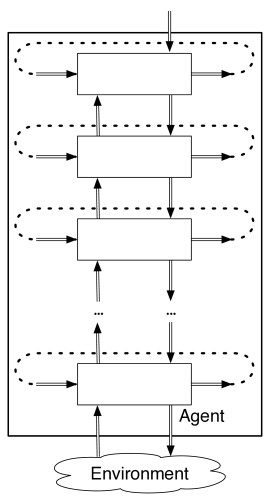
\includegraphics[scale=.5]{architettura1.png}
\caption{Architettura interazione tra agenti}
\end{center}
\end{figure}
\begin{figure}[h!]
\begin{center}
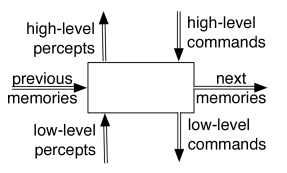
\includegraphics[scale=.65]{architettura2.png}
\caption{Architettura interna di un agente}
\end{center}
\end{figure}
Un'architettura di sistema di agenti gerarchici idealizzata. I rettangoli senza etichetta rappresentano i livelli e le linee doppie rappresentano il flusso di informazioni. Le linee tratteggiate mostrano come l'output in una volta sia l'input per la volta successiva. Ogni livello vede gli strati sottostanti come un corpo virtuale da cui riceve le percezioni ea cui invia comandi. L' orizzonte progettualeal livello inferiore è molto più breve dell'orizzonte di pianificazione ai livelli superiori. Gli strati di livello inferiore funzionano molto più velocemente, reagiscono a quegli aspetti del mondo a cui è necessario reagire rapidamente e offrono una visione più semplice del mondo agli strati superiori, nascondendo dettagli che non sono essenziali per gli strati superiori. Le persone devono reagire al mondo, al livello più basso, in frazioni di secondo, ma pianificare al livello più alto anche per decenni nel futuro. Ad esempio, il motivo per frequentare un determinato corso universitario potrebbe essere la carriera a lungo termine.In un controller gerarchico possono esserci più canali, ognuno dei quali rappresenta una caratteristica, tra i livelli e tra i livelli in momenti diversi. Ci sono tre tipi di input per ogni livello alla volta:
\begin{itemize}
\item le caratteristiche che provengono dallo stato di credenza, a cui si fa riferimento come valori ricordati o precedenti di queste caratteristiche
\item le caratteristiche che rappresentano le percezioni dal livello sottostante nella gerarchia
\item le caratteristiche che rappresentano i comandi dal livello superiore nella gerarchia.
\end{itemize} 

Ci sono tre tipi di output per ogni lievello alla volta: le percezioni di alto livello del livello superiore, i comandi di basso livello per il livello sottostante e i valori successivi per le caratteristiche dello stato di credenza. Un'implementazione di un livello specifica in che modo gli output di un livello sono una funzione dei suoi input. La definizione della funzione di transizione dello stato di convinzione e della funzione di comando può essere estesa per includere comandi di livello superiore come input e ogni livello richiede anche una funzione di percezione , rappresentata come di seguito . Quindi un livello implementa:
\begin{center}
$transizione: S \times P_l \times C_h \rightarrow S$

$comando: S \times P_l \times C_h \rightarrow C_l$

$raccontare: S \times P_l \times C_h \rightarrow P_h$
\end{center}
dove \textit{S} è lo stato di credenza, $C_h$ è l'insieme dei comandi del livello superiore, $P_l$ è l'insieme delle percezioni dello strato inferiore, $C_l$ è l'insieme dei comandi per il livello inferiore, $P_h$ è l'insieme delle percezioni per lo strato superiore. Il calcolo di queste funzioni può comportare un calcolo arbitrario, ma l'obiettivo è mantenere ogni livello il più semplice possibile. Per implementare un controller, ogni input a un livello deve ottenere il suo valore da qualche parte. Ogni input di percezione o comando dovrebbe essere collegato a un output di un altro livello. Altri input provengono dalle credenze ricordate. Le uscite di un livello non devono essere collegate a nulla, oppure potrebbero essere collegate a più ingressi. Il ragionamento di alto livello, come svolto negli strati superiori, è spesso discreto e qualitativo, mentre il ragionamento di basso livello, come svolto negli strati inferiori, è spesso continuo e quantitativo (vedi riquadro ). Un controllore che ragiona in termini di valori sia discreti che continui è chiamato sistema ibrido.

Gran parte della scienza e dell'ingegneria considera \textbf{il ragionamento quantitativo} con quantità numeriche, utilizzando il calcolo differenziale e integrale come strumenti principali. \textbf{Il ragionamento qualitativo} è il ragionamento, spesso usando la logica, sulle distinzioni qualitative piuttosto che sui valori numerici per determinati parametri. Il ragionamento qualitativo è importante per una serie di ragioni:
\begin{itemize}
\item Un agente potrebbe non sapere quali sono i valori esatti.
\item Il ragionamento può essere applicabile indipendentemente dai valori quantitativi.
\item Un agente deve fare un ragionamento qualitativo per determinare quali leggi quantitative sono applicabili.
\end{itemize}
Il ragionamento qualitativo utilizza valori discreti, che possono assumere diverse forme:
\begin{itemize}
\item I punti di riferimento sono valori che fanno distinzioni qualitative nell'individuo modellato.
\item Il ragionamento per ordini di grandezza implica un ragionamento approssimativo che ignora le distinzioni minori.
\item I derivati qualitativi indicano se un valore sta aumentando, diminuendo o rimanendo invariato.
\end{itemize}

Un agente flessibile ha bisogno di fare ragionamento qualitativo prima di fare ragionamento quantitativo. A volte il ragionamento qualitativo è tutto ciò che serve. Pertanto, un agente non ha sempre bisogno di fare un ragionamento quantitativo, ma a volte ha bisogno di fare sia un ragionamento qualitativo che quantitativo.

\subsubsection{Agire con ragionamento}

Per un agente intelligente, lo stato di credenza può essere complesso, anche per un singolo strato. La definizione di uno stato di credenza è molto generale e non vincola ciò che dovrebbe essere ricordato dall'agente. Spesso è utile che l'agente mantenga qualche modello del mondo, anche se il suo modello è incompleto e impreciso. Un modello di mondo è una rappresentazione dello stato del mondo in un momento particolare e/o delle dinamiche del mondo. Ad un estremo, un modello può essere così valido che l'agente può ignorarne le percezioni. L'agente può quindi determinare cosa fare semplicemente ragionando. Questo approccio richiede un modello sia dello stato del mondo che delle dinamiche del mondo. Dato lo stato in una volta e la dinamica, è possibile prevedere lo stato nella volta successiva. Questo processo è noto come dead reckoning.  Quando il mondo è dinamico o quando ci sono attuatori rumorosi, il rumore si accumula, così che le stime di posizione diventano presto così imprecise che sono inutili. Tuttavia, se il modello è accurato a un certo livello di dettaglio, potrebbe comunque essere utile. All'altro estremo c'è un sistema puramente reattivo che basa le sue azioni sulle percezioni, ma non aggiorna il suo stato di credenza interna. La funzione di comando in questo caso è una funzione dai percetti alle azioni. Un approccio più promettente consiste nel combinare la previsione dell'agente dello stato mondiale con il rilevamento delle informazioni. Questo può assumere diverse forme:
\begin{itemize}
\item Se vengono modellati sia il rumore della previsione in avanti che il rumore del sensore, il successivo stato di credenza può essere stimato utilizzando la regola di Bayes. Questo è noto come filtraggio.
\item Con sensori più complicati come la visione, un modello può essere utilizzato per prevedere dove è possibile trovare le caratteristiche visive, quindi la visione può essere utilizzata per cercare queste caratteristiche vicino alla posizione prevista. Ciò rende il compito di visione molto più semplice e la visione può ridurre notevolmente gli errori di posizione derivanti dalla sola previsione in avanti.
\end{itemize}
Un problema di controllo è separabile se è possibile ottenere l'azione migliore trovando prima il miglior modello del mondo e quindi utilizzando quel modello per determinare l'azione migliore. Sfortunatamente, la maggior parte dei problemi di controllo non sono separabili. Ciò significa che l'agente deve considerare più modelli per determinare cosa fare. Di solito, non esiste un "modello migliore" al mondo che sia indipendente da ciò che l'agente farà con il modello.

L'esperienza nello studio e nella costruzione di agenti intelligenti ha dimostrato che un agente intelligente richiede una rappresentazione interna del suo stato di credenza. \textbf{La conoscenza} è l'informazione su un dominio che viene utilizzata per agire in quel dominio. La conoscenza può includere conoscenze generali che possono essere applicate a situazioni particolari, nonché credenze su uno stato specifico. \textbf{Un sistema basato sulla conoscenza} è un sistema che utilizza la conoscenza di un dominio per agire o risolvere problemi. Conoscenza tende a significare informazioni generali e persistenti che vengono considerate vere per un periodo di tempo più lungo. La credenza tende a significare informazioni più transitorie che vengono riviste sulla base di nuove informazioni. Spesso la conoscenza e le credenze vengono con le misure di quanto dovrebbero essere credute. In un sistema di intelligenza artificiale, la conoscenza in genere non è necessariamente vera ed è giustificata solo come utile. La distinzione tra conoscenza e credenza spesso diventa offuscata quando un modulo di un agente può trattare alcune informazioni come vere, ma un altro modulo può essere in grado di rivedere tali informazioni.

\begin{figure}[h!]
\begin{center}
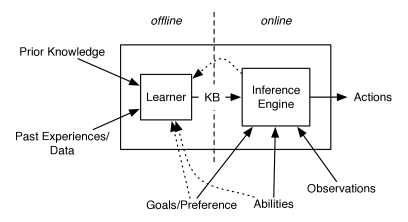
\includegraphics[scale=0.9]{scomposizione.png}
\caption{Differenza tra stato online e offline}
\end{center}
\end{figure}

Una base di conoscenza , KB, viene creata offline da uno studente e viene utilizzata online per determinare le azioni. Questa decomposizione di un agente è ortogonale alla vista a strati di un agente; un agente intelligente richiede sia un'organizzazione gerarchica che basi di conoscenza. \textbf{Online}, quando l'agente agisce, l'agente usa la sua base di conoscenza, le sue osservazioni del mondo, i suoi obiettivi e le sue capacità per scegliere cosa fare e per usare le informazioni appena acquisite per aggiornare la sua base di conoscenza. \textbf{La base di conoscenza} è la \textbf{sua memoria a lungo termine}, dove conserva le conoscenze necessarie per agire in futuro. Questa conoscenza viene appresa da conoscenze pregresse e da dati ed esperienze passate. \textbf{Lo stato di convinzione} è \textbf{la memoria a breve termine} dell'agente, che mantiene il modello dell'ambiente attuale necessario tra le fasi temporali. \textbf{Offline}, prima che l'agente debba agire, l'agente utilizza le conoscenze pregresse e le esperienze passate (le proprie esperienze passate o i dati che gli sono stati forniti) in quello che viene chiamato \textbf{apprendimento} per costruire una base di conoscenza utile per agire online. I ricercatori hanno tradizionalmente considerato il caso che coinvolge molti dati e conoscenze pregresse molto generali, o addirittura non informative, nel campo della statistica. Il caso di una ricca conoscenza pregressa e di pochi o nessun dato da cui apprendere è stato studiato sotto l'ombrello di sistemi esperti . Per la maggior parte dei domini non banali, l'agente ha bisogno di tutte le informazioni disponibili, quindi richiede sia una ricca conoscenza preliminare che osservazioni da cui imparare. Gli obiettivi e le abilità vengono forniti offline, online o entrambi, a seconda dell'agente. Il calcolo online può essere reso più efficiente se la base di conoscenze è ottimizzata per gli obiettivi e le abilità particolari. Questo spesso non è possibile quando gli obiettivi e le abilità sono disponibili solo in fase di esecuzione.

La base di conoscenza richiesta per il calcolo online può essere creata inizialmente in fase di progettazione e quindi aumentata offline dall'agente. Un'ontologia è una teoria su ciò che esiste, o ciò che può esistere, in un particolare dominio. In AI, \textbf{un'ontologia} è una specificazione del significato dei simboli utilizzati in un sistema informativo, dove i simboli si riferiscono a cose che esistono. Un'ontologia specifica ciò che esiste e il vocabolario utilizzato per descrivere ciò che esiste. Nel caso più semplice, se un agente utilizza una rappresentazione esplicita basata sullo stato con piena osservabilità, un'ontologia specifica la mappatura tra lo stato e il mondo. In altri casi, un'ontologia definirebbe le caratteristiche o gli individui e le relazioni. L'ontologia viene logicamente prima dei dati e della conoscenza a priori: abbiamo bisogno di un'ontologia per avere dati o per avere conoscenza. Senza un'ontologia, i dati sono solo sequenze di bit. Senza un'ontologia, un essere umano non sa cosa inserire; è l'ontologia che specifica il significato dei dati. L'ontologia specifica un livello, o livelli, di astrazione. Se l'ontologia cambia, i dati devono cambiare. La base di conoscenza è in genere costruita offline da una combinazione di conoscenze e dati esperti. Un ingegnere della conoscenza è una persona che interagisce con un esperto di dominio per costruire una base di conoscenza. L'ingegnere della conoscenza conosce i sistemi intelligenti, ma non necessariamente il dominio, e l'esperto di dominio conosce il dominio, ma non necessariamente come specificare la conoscenza. Offline, l'agente può combinare le conoscenze degli esperti e tutti i dati disponibili. Ad esempio, può compilare parti della base di conoscenza per consentire un'inferenza più efficiente. Offline, il sistema può essere testato e sottoposto a debug.

Online , le informazioni sulla situazione particolare diventano disponibili e l'agente deve agire. Le informazioni includono le osservazioni del dominio e spesso le preferenze o gli obiettivi. L'agente può ottenere osservazioni da sensori, utenti e altre fonti di informazioni, come siti Web, sebbene in genere non abbia accesso agli esperti di dominio o all'ingegnere della conoscenza durante l'azione. Un agente in genere ha molto più tempo per il calcolo offline che per il calcolo online. Durante il calcolo online può trarre vantaggio da obiettivi particolari e osservazioni particolari. Offline, può acquisire conoscenze su come interagiscono malattie e sintomi ed eseguire il debug e la compilazione. Può solo eseguire il calcolo su un particolare paziente online. Online sono coinvolti i seguenti ruoli:
\begin{itemize}
\item  \textbf{Un utente} è una persona che ha bisogno di esperienza o ha informazioni su situazioni individuali. Gli utenti in genere non sono esperti nel dominio della knowledge base. Spesso non sanno quali informazioni sono necessarie al sistema. Pertanto, è irragionevole aspettarsi che si offra volontariamente tutto ciò che è vero su una particolare situazione. Deve essere fornita un'interfaccia semplice e naturale poiché gli utenti in genere non comprendono la struttura interna del sistema. Gli utenti spesso, tuttavia, devono prendere decisioni informate sulla base della raccomandazione del sistema; pertanto, richiedono una spiegazione del motivo per cui la raccomandazione è appropriata.
\item \textbf{I sensori} forniscono informazioni sull'ambiente. I sensori sono disponibili in due varietà principali. Un sensore passivo fornisce continuamente informazioni all'agente. I sensori passivi includono termometri, fotocamere e microfoni. Il progettista può in genere scegliere dove si trovano i sensori o dove stanno puntando, ma si limitano a fornire le informazioni sull'agente. Al contrario, un sensore attivo è controllato o interrogato per informazioni.
\item  \textbf{Una fonte di conoscenza esterna}, come un sito Web o un database, potrebbero essere poste domande e può fornire la risposta per un dominio limitato. Un agente può chiedere a un sito Web meteo per la temperatura in un luogo particolare o al sito Web di una compagnia aerea per l'orario di arrivo di un particolare volo. Le fonti di conoscenza hanno vari protocolli e compromessi di efficienza. L'interfaccia tra un agente e una fonte di conoscenza esterna è chiamata wrapper. Un wrapper traduce tra la rappresentazione utilizzata dall'agente e le query che la fonte di conoscenza esterna è pronta a gestire. Spesso i wrapper sono progettati in modo che l'agente sia in grado di porre la stessa query a più fonti di conoscenza
\end{itemize}

\newpage

\subsection{Capitolo 3 - Ricerca di soluzioni}

\begin{center}
Hai mai visto un granchio sulla riva che strisciava all'indietro alla ricerca dell'Oceano Atlantico e scompare? Questo è il modo in cui opera la mente dell'uomo.

HL Mencken 
\end{center}

Il capitolo precedente ha discusso di come un agente percepisce e agisce, ma non di come i suoi obiettivi influenzano le sue azioni. Un agente potrebbe essere programmato per agire nel mondo per raggiungere un obiettivo prefissato o una serie di obiettivi, ma in tal caso non si adatterebbe a obiettivi mutevoli e quindi non sarebbe intelligente. Un agente intelligente ha bisogno di ragionare sulle sue capacità e sui suoi obiettivi per determinare cosa fare. Questo capitolo definisce il problema di un agente che decide come risolvere un obiettivo come il problema della ricerca di un percorso in un grafico. Presenta diversi modi per risolvere tali problemi su un computer.

\subsubsection{Risoluzione dei problemi come ricerca}

Nel caso più semplice in cui un agente decide cosa dovrebbe fare, l'agente ha un modello del mondo basato sullo stato, con un obiettivo da raggiungere e nessuna incertezza. Questa è una rappresentazione piatta (non gerarchica) o un singolo livello di una gerarchia. L'agente è in grado di determinare come raggiungere il suo obiettivo cercando nella sua rappresentazione dello spazio un modo per passare dal suo stato attuale a uno stato che soddisfi il suo obiettivo. Dato un modello completo, cerca di trovare una sequenza di azioni che raggiungano il suo obiettivo prima di dover agire nel mondo. Questo problema può essere astratto dal problema matematico di trovare un percorso dal nodo iniziale a un nodo obiettivo in un grafo orientato.

Trovare il percorso migliore da una posizione corrente a una destinazione è un problema di ricerca. Lo stato include la posizione e possibilmente la direzione di marcia e la velocità. Il miglior percorso potrebbe significare trovare il percorso più breve (a distanza minore), il percorso più veloce, il percorso più economico che tiene conto di tempo, denaro (ad es. carburante e pedaggi) e dell'attrattiva del percorso. Trovare il percorso più breve è generalmente più facile da implementare poiché il calcolo delle distanze da una mappa è generalmente semplice. Trovare il percorso migliore che tenga conto delle altre preferenze che le persone potrebbero avere è complicato. È difficile acquisire queste preferenze e le persone potrebbero non essere nemmeno in grado di articolare queste preferenze e compromessi. Ma date le preferenze, il problema si riduce a quello della ricerca, seppur con una complessa funzione di costo.

Questa nozione di ricerca è un calcolo esclusivamente all'interno dell'agente. È diverso dalla ricerca nel mondo, quando un agente potrebbe dover agire nel mondo, ad esempio un robot che cerca chiavi, solleva cuscini e così via. È anche diverso dalla ricerca sul Web, che implica la ricerca di informazioni indicizzando enormi quantità di dati e cercando di trovare la risposta migliore per ogni query di ricerca. Cercare in questo capitolo significa cercare in una rappresentazione interna un percorso verso un obiettivo. La ricerca è alla base di gran parte dell'intelligenza artificiale. Quando a un agente viene assegnato un problema, di solito gli viene fornita solo una descrizione che gli consente di riconoscere una soluzione, non un algoritmo per risolverlo. Deve cercare una soluzione. L'esistenza di problemi NP-completi , con mezzi efficienti per riconoscere le soluzioni ma senza metodi efficienti per trovarle, indica che la ricerca è una parte necessaria della risoluzione dei problemi.

\subsubsection{Spazio di stato}

Una formulazione generale dell'azione intelligente è in termini di \textbf{spazio di stato}. \textbf{Uno stato} contiene tutte le informazioni necessarie per prevedere gli effetti di un'azione e per determinare se uno stato soddisfa l'obiettivo. La ricerca nello spazio degli stati presuppone:

\begin{itemize}
\item L'agente ha una perfetta conoscenza dello spazio degli stati e sta pianificando il caso in cui osserva in quale stato si trova: c'è piena osservabilità.
\item L'agente ha una serie di azioni che hanno effetti deterministici noti.
\item L'agente può determinare se uno stato soddisfa l'obiettivo.
\end{itemize}
\textbf{Una soluzione} è una sequenza di azioni che porterà l'agente dal suo stato attuale a uno stato che soddisfa l'obiettivo. Un problema nello spazio degli stati è costituito da:
\begin{itemize}
\item un insieme di stati
\item uno stato distinto chiamato \textbf{stato iniziale}
\item per ogni stato, un insieme di azioni disponibili per l'agente in quello stato
\item \textbf{una funzione di azione} che, dati uno stato e un'azione, restituisce un nuovo stato
\item \textbf{un obiettivo} specificato come funzione booleana, $obiettivo(S)$, che è vera quando lo stato \textit{S} soddisfa l'obiettivo e in tal caso diciamo che \textit{S} è \textbf{stato obiettivo}.
\item un criterio che specifica la qualità di una soluzione accettabile. Una soluzione che è la migliore secondo alcuni criteri è chiamata soluzione ottima.
\end{itemize}

\subsubsection{Ricerca nel grafo}
il problema di trovare una sequenza di azioni per raggiungere un obiettivo è astratto come la ricerca di percorsi in grafi diretti. Per risolvere un problema, definire prima lo spazio di ricerca sottostante e quindi applicare un algoritmo di ricerca a tale spazio di ricerca. Molte attività di problem solving sono trasformabili nel problema di trovare un percorso in un grafico. La ricerca nei grafici fornisce un modello astratto appropriato di risoluzione dei problemi indipendente da un particolare dominio. Un grafo diretto è costituito da un insieme di nodi e da un insieme di archi diretti tra i nodi. L'idea è di trovare un percorso lungo questi archi dal nodo iniziale a un nodo obiettivo. Nella rappresentazione di un problema nello spazio degli stati, gli stati sono rappresentati come nodi e le azioni come archi. L'astrazione è necessaria perché potrebbe esserci più di un modo per rappresentare un problema come grafico.
\subsubsection{Formalizzazione della ricerca nei grafici}
Un \textbf{grafo orientato} è costituito da un insieme di \textit{N} \textbf{nodi} e un insieme \textit{A} di archi, dove \textbf{un arco} è una coppia ordinata di nodi. In questa definizione, un nodo potrebbe essere qualsiasi cosa. Ci possono essere infiniti nodi e archi. Non assumiamo che un grafo sia rappresentato in modo esplicito; richiediamo solo una procedura per generare nodi e archi secondo necessità. L'arco $<n_1 , n_2 >$ è un arco uscente da $n_1$ ed è un arco in arrivo in $n_2$. Un nodo $n_2$ è un vicino di $n_1$ se c'è un arco da $n_1$ a $n_2$; cioè se $< n_1 , n_2 > \in A$. Il concetto di vicinanza è un concetto asimmetrico. Inoltre gli archi possono essere etichettati. Un \textbf{percorso} dal nodo \textit{S} al nodo \textit{g} è una sequenza di nodi $< n_1 , n_2, \dots, n_k >$ tale che $S = n_0 $, $g = n_k$, e $<n_{i-1},n_i> \in A$, cioè, c'è un arco da $n_{i-1}$ a $n_i$. Un \textbf{obiettivo} è una funzione booleana sui nodi. Se $obiettivo(n)$ è vero, diciamo che il nodo \textit{n} soddisfa l'obiettivo, e possiamo definirlo come \textbf{nodo obiettivo}.

A volte c'è un costo associato agli archi. Scriviamo il costo dell'arco $< n_i,n_j>$ come $costo(<n_i,nj>)$. I costi degli archi inducono un costo dei cammini. Dato un percorso $p=<n_0,n_1,\dots,n_k>$ il costo del percorso \textit{p} è la somma dei costi degli archi del percorso:
\begin{center}
$costo(p)= \sum_{i=0}^K costo(<n_{i-1},n_i> )$
\end{center}

Una \textbf{soluzione ottimale} è una delle soluzioni che ha il costo più basso. Cioè, una soluzione ottimale è un percorso \textit{p} dal nodo iniziale a un nodo obiettivo in modo tale che non vi sia alcun percorso $p'$ dal nodo iniziale a un nodo obiettivo dove $costo(p')<costo(p)$. Un \textbf{ciclo} è un percorso non vuoto in cui il nodo finale è lo stesso del nodo iniziale, ovvero $<n_0,n_1,\dots,n_k>$ tale che $n_0=n_k$. Un grafo diretto senza cicli è chiamato \textbf{grafo aciclico diretto (DAG)}. Un \textbf{albero} è un DAG in cui c'è un nodo senza archi in entrata e ogni altro nodo ha esattamente un arco in entrata. Il nodo senza archi in entrata è definito radice dell'albero. Un nodo senza archi uscenti è chiamato foglia. In un albero, i nodi neighboor sono chiamati anche figli. In molti problemi il grafico i ricerca non è fornito in modo esplicito, ma è costruito dinamicamente secondo necessità. Il \textbf{fattore di ramificazione in avanti} di un nodo è il numero di archi in uscita dal nodo. Il \textbf{fattore di ramificazione all'indietro} di un nodo è il numero di archi in ingresso al nodo. Questi fattori forniscono misure per la complessità degli algoritmi dei grafi. 


\subsubsection{Algoritmo di ricerca generico}

In questa sezione descriviamo un algoritmo i ricerca generico.
\begin{figure}[h!]
\begin{center}
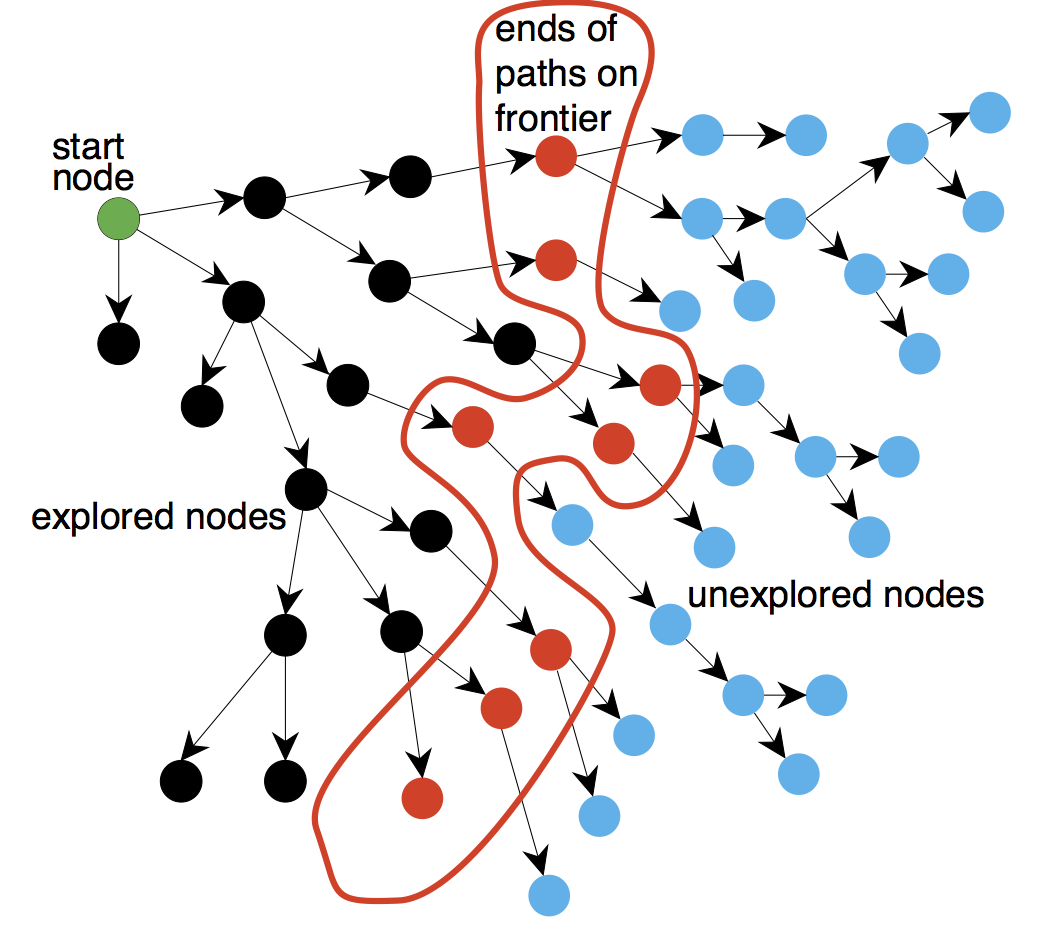
\includegraphics[scale=0.4]{algoritmoDiRicerca.png}
\caption{Algoritmo di ricerca generico}
\end{center}
\end{figure}

L'idea intuitiva alla base dell'algoritmo di ricerca generico, dato un grafo, un nodo iniziale e un obiettivo, è esplorare i percorsi in modo incrementale dal nodo iniziale. Questo viene fatto mantenendo una frontiera (o frangia ) di percorsi dal nodo iniziale. La frontiera contiene tutti i percorsi che potrebbero formare segmenti iniziali di percorsi dal nodo iniziale a un nodo obiettivo.  Inizialmente, la frontiera contiene il percorso banale contenente solo il nodo iniziale e nessun arco. Man mano che la ricerca procede, la frontiera si espande nei nodi inesplorati fino a quando non si incontra un nodo obiettivo. Diverse strategie di ricerca si ottengono fornendo un'adeguata implementazione della frontiera.
\begin{lstlisting}
procedura Cerca(G,S,obiettivo)
	Input
	G: grafo con N nodi e A archi
	S: nodo di partenza
	obiettivo: funzione booleana di nodi
	Output
	percorso da S a un nodo per il quale l'obiettivo e' vero o
	null se non ci sono percorsi 
	Locale
	Frontiera: insieme di percorsi
	Frontiera ={<S>}
	 mentre (Frontiera != insieme vuoto ) == false
	 	seleziona e rimuovi <n0,...,nk> da Frontiera
	 	se obbiettivo (nk) allora
	 		ritorno <n0,...,nk>
	 	Frontiera= Frontiera unito a {<n0,..,nk,n> : <nk,n> appartiene a A}
	ritorno vuoto
\end{lstlisting}

La frontiera è un insieme di percorsi. Inizialmente, la frontiera contiene il percorso a costo zero costituito solo dal nodo iniziale. Ad ogni passaggio, l'algoritmo rimuove un percorso $<n_0,...,n_k>$ dalla frontiera. Se $obbiettivo(n_k)$ è vero (cioè $n_k$ è un nodo obiettivo), ha trovato una soluzione e restituisce il percorso $<n_0,...,n_k>$. Altrimenti, il percorso viene esteso di un altro arco trovano i vicini di $n_k$. Per ogni vicino i n di $n_k$, il sentiero $<n_0,...,n_k,n>$ si aggiunge alla frontiera. Questo passaggio è noto come espansione del percorso. Alcune caratteristiche importanti i questo algoritmo sono: \begin{itemize}
\item Il percorso scelto alla riga 13 determina la strategia di ricerca. La selezione di un percorso può influire sull'efficienza.
\item E' utile pensare a un valore di ritorno, presente nella riga 15, come un ritorno temporaneo, in cui un chiamante può riprovare la ricerca per ottenere un'altra risposta.
\item Se la procedura ritorna vuoto, non ci sono soluzioni o non ci sono soluzioni rimanenti se la ricerca è stata ripetuta.
\item l'algoritmo verifica solo se un percorso termina in un nodo obiettivo dopo che il percorso è stato selezionato dalla frontiera, non quando viene aggiunto ad essa. Ci sono due ragioni importanti per questo. Potrebbe esserci un costoso arco da un nodo sulla frontiera a un nodo obiettivo. La ricerca non dovrebbe sempre restituire il percorso con questo arco, perché potrebbe esistere una soluzione a basso costo. Questo è fondamentale quando è richiesto il percorso più economico. Un secondo motivo è che può essere costoso determinare se un nodo è un nodo obiettivo, quindi questo dovrebbe essere ritardato nel caso in cui il calcolo non sia necessario.
\end{itemize}

Se il nodo alla fine del percorso selezionato non è un nodo obiettivo e non ha vicini, estendere il percorso significa rimuovere il percorso dalla frontiera. Questo risultato è ragionevole perché questo percorso non può essere parte di un percorso dal nodo iniziale a un nodo obiettivo. 

Di solito, gli algoritmi \textbf{non sono deterministici}, il che significa che ci sono scelte nel programma che non vengono specificate. Esistono due forme di non determinismo:
\begin{itemize}
\item \textbf{"don't care non-determinism"}, se una selezione non porta a una soluzione, nemmeno le altre selezioni lo faranno. Il non determinismo non interessa viene utilizzato nell'allocazione delle risorse, in cui si verifica un numero di richieste per un numero limitato di risorse e un algoritmo di pianificazione deve selezionare chi ottiene quale risorsa in ogni momento. La correttezza non dovrebbe essere influenzata dalla selezione, ma l'efficienza e la risoluzione potrebbero esserlo. Quando c'è una sequenza infinita di selezioni, un meccanismo di selezione è giusto se alla fine verrà selezionata una richiesta che è ripetutamente disponibile per essere selezionata. Il problema di un elemento che viene ripetutamente non selezionato è chiamato fame . In questo contesto, un'euristica è una regola pratica che può essere utilizzata per selezionare un valore.
\item Nel non-determinismo , solo perché una scelta non ha portato a una soluzione non significa che altre scelte non lo faranno. Spesso si parla di un oracolo che potrebbe specificare, in ogni punto, quale scelta porterà a una soluzione. Poiché il nostro agente non ha un tale oracolo, deve cercare nello spazio delle scelte alternative.
\end{itemize}

\subsubsection{Strategie di ricerca non informate}

Un problema determina il grafico, il nodo iniziale e l'obiettivo ma non quale percorso selezionare dalla frontiera. Questo è il compito di una \textbf{strategia di ricerca}. Una strategia di ricerca definisce l'ordine in cui i percorsi vengono selezionati dalla frontiera. Diverse strategie si ottengono modificando il modo in cui viene attuata la selezione dei percorsi di frontiera. Nelle \textbf{strategie di ricerca non informate} non tengono conto della posizione dell'obiettivo. Questi algoritmi ignorano dove stanno andando finché non trovano un obiettivo e segnalano il successo.

Nella ricerca \textbf{in ampiezza} la frontiera viene implementata come una coda FIFO. Pertanto, il percorso selezionato dalla frontiera è quello che è stato aggiunto per primo. Questo approccio implica che i percorsi dal nodo iniziale siano generati in base al numero di archi nel percorso. Ad ogni iterazione viene selezionato uno dei percorsi con il minor numero di archi.

\begin{figure}[h!]
\begin{center}
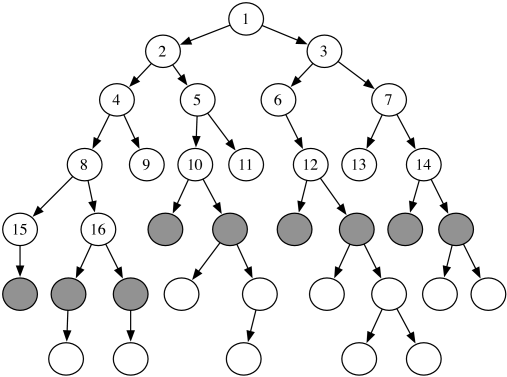
\includegraphics[scale=0.5]{ricercaAmpiezza.png}
\caption{Algoritmo di ricerca in ampiezza}
\end{center}
\end{figure}

Supponiamo che il fattore di ramificazione della ricerca sia \textit{b}. Se il prossimo percorso da selezionare sulla frontiera contiene \textit{n} archi, allora ci sono almeno $b^{n-1}$ elementi di frontiera. Tutti questi percorsi contengono \textit{n} o $n+1$ archi. Pertanto, sia la complessità spaziale che temporale sono esponenziali nel numero di archi del percorso verso un obiettivo con il minor numero di archi. Questo metodo è garantito per trovare una soluzione se esiste e troverà una soluzione con il minor numero di archi. La ricerca in ampiezza è utile quando il problema è abbastanza piccolo in modo che lo spazio non sia un problema e si vuole che una soluzione contenga il minor numero di archi. È un metodo scadente quando tutte le soluzioni hanno molti archi o è disponibile una certa conoscenza euristica. Non viene utilizzato molto spesso per problemi di grandi dimensioni in cui il grafo viene generato dinamicamente a causa della sua complessità spaziale esponenziale.

Nella \textbf{ricerca in profondità}, la frontiera si comporta come una pila di percorsi LIFO. In una pila, gli elementi vengono aggiunti e rimossi dalla cima della pila. Usare una pila significa che il percorso selezionato e rimosso dalla frontiera in qualsiasi momento è l'ultimo percorso aggiunto.

\begin{figure}[h!]
\begin{center}
\includegraphics[scale=0.5]{ricercaProfondità.png}
\caption{Algoritmo di ricerca in profondità}
\end{center}
\end{figure}

L'implementazione della frontiera come stack fa sì che i percorsi vengano perseguiti in modo approfondito, cercando un percorso fino al suo completamento prima di provare un percorso alternativo. Si dice che questo metodo implichi il backtracking : l'algoritmo seleziona una prima alternativa su ciascun nodo e torna indietro all'alternativa successiva quando ha perseguito tutti i percorsi dalla prima selezione. Alcuni percorsi possono essere infiniti quando il grafico ha cicli o infiniti nodi, nel qual caso una ricerca in profondità potrebbe non interrompersi mai. Questo algoritmo non specifica l'ordine in cui i percorsi dei vicini vengono aggiunti alla frontiera. L'efficienza dell'algoritmo è sensibile a questo ordinamento. Se c'è una soluzione sul primo ramo cercato, la complessità temporale è lineare nel numero di archi nel percorso. Nel peggiore dei casi, la ricerca in profondità può rimanere intrappolata su rami infiniti e non trovare mai una soluzione, anche se esiste, per grafi infiniti o per grafi con cicli. Se il grafo è un albero finito, con il fattore di ramificazione in avanti minore o uguale a b e tutti i percorsi hanno dall'inizio k o meno archi, il caso peggiore di complessità temporale è $O(b^k)$.

Poiché la ricerca in profondità è sensibile all'ordine in cui i vicini vengono aggiunti alla frontiera, è necessario prestare attenzione a farlo in modo sensato. Questo ordinamento può essere eseguito staticamente (in modo che l'ordine dei vicini sia fisso) o dinamico (dove l'ordine dei vicini dipende dall'obiettivo). La ricerca in profondità è appropriata quando lo spazio è limitato, esistono molte soluzioni o l'ordine in cui i vicini di un nodo vengono aggiunti allo stack può essere ottimizzato in modo da trovare soluzioni al primo tentativo. E' un metodo scadente quando è possibile rimanere intrappolati in percorsi infiniti, cosa che si verifica quando il grafico è infinito o quando ci sono cicli nel grafico, esistono soluzioni a poca profondità, perché in questo caso la ricerca può esplorare molti percorsi lunghi prima di trovare le soluzioni brevi o ci sono più percorsi per un nodo. La ricerca in profondità è la base per una serie di altri algoritmi, come l'approfondimento iterativo.

La ricerca in ampiezza, che garantisce che verrà trovato un percorso, richiede uno spazio esponenziale. La ricerca in profondità potrebbe non interrompersi su grafici infiniti o grafici con cicli. Un modo per combinare l'efficienza spaziale della ricerca in profondità con l'ottimalità della ricerca in ampiezza consiste nell'usare \textbf{l' approfondimento iterativo}. L'idea è di ricalcolare gli elementi della frontiera in ampiezza piuttosto che memorizzarli. Ogni ricalcolo può essere una ricerca in profondità, che quindi utilizza meno spazio. La ricerca iterativa chiama ripetutamente un \textbf{depth-bounded searcher} (ricercatore con limite di profondità), questo accetta un \textbf{depth bound} (limite di profondità) e non esplora mai percorsi con più archi rispetto a questo limite. L'approfondimento iterativo prima esegue una ricerca in profondità fino alla profondità 1 costruendo percorsi di lunghezza 1 in modo approfondito. Se ciò non trova una soluzione, può costruire percorsi alla profondità 2, quindi alla profondità 3 e così via fino a quando non viene trovata una soluzione. Quando una ricerca con limite di profondità n non riesce a trovare una soluzione, può eliminare tutto il calcolo precedente e ricominciare con un limite di profondità di n+1. Alla fine, troverà una soluzione, se esiste, e, poiché enumera i percorsi in base al numero di archi, verrà sempre trovato per primo un percorso con il minor numero di archi.

Per garantire che si fermi per i grafi finiti, la ricerca iterativa di approfondimento deve distinguere tra fallimento perché è stato raggiunto il limite di profondità e fallimento dovuto all'esaurimento dello spazio di ricerca. Nel primo caso, la ricerca deve essere ripetuta con un limite di profondità maggiore. Nel secondo caso, è una perdita di tempo riprovare con un limite di profondità maggiore, perché non esiste alcun percorso, non importa quale sia la profondità, e quindi l'intera ricerca dovrebbe fallire.

\begin{lstlisting}
procedure ID-Search(G,s,goal)
Input
	G: grafo con N nodi e A archi
	s: nodo di partenza
	goal: funzione Booleana sui nodi
Output
	percorso da s a un nodo per il quale il goal e' verificato 
	o viene restituito il simbolo(* $\bot $ *) per indicare che non vi e' nessun percorso
Local
	hit_depth_bound : Boolean
	bound: integer
	procedure Depth_bounded_search((*$<n_0,\dots,n_k>$*),b)
	
		Input
		(*$<n_0,\dots,n_k>$*): il percorso
		b: nomero intero maggiore di 0
		
		Output
		percorso verso la meta di lunghezza K+b se ne esiste uno
		
		se (*$b>0$*)
			allora per ogni (*$arco<n_K,n> \in A$*)
			 res:= DEpth_bounded_search( (* $ <n_0,...,n_k,n> $ *),b-1)
			 se res e' un percorso allora
			 	ritorna res
			 altrimenti se obiettivo((*$n_k$*) allora
			 	ritorna (*$<n_0,...,n_k>$*)
			 altrimenti se (*$n_k$*) ha dei vicini allora
			 	hit_depth_bound:= true
			bound:=0
		repeat
			hit_depth_bound :=false
			res:= Depth_bounded_search((*$<s>$*),bound)
			se res e' un percorso allora
				ritorna res
			bound = bound+1
	until not hit_depth_bound
		
\end{lstlisting}

Questo é lo pseudocodice per la ricerca di approfondimento iterativo, ID-Search. La procedura locale Depth-bounded-search implementa una ricerca in profondita' limitata alla profondita' (usando la ricorsione per mantenere lo stack) che pone un limite alla lunghezza dei percorsi per i quali sta cercando. Restituisce un percorso o raggiunge la fine del suo codice e ritorna senza percorso. Utilizza una ricerca in profondità per trovare percorsi di lunghezza K+b, dove K é la lunghezza del percorso dato dall'inizio e b é un numero intero non negativo. Il ricercatore iterativo di approfondimento chiama Depth-bounded-search per aumentare i limiti di profondita'. Questo programma trova i percorsi dei nodi obiettivo nello stesso ordine della ricerca in ampiezza, Ha solo bisogno di controllare un obiettivo quando b=0, perché sa che non ci sono soluzioni per i limiti inferiori.

Per garantire che la ricerca di approfondimento iterativo fallisca ogni volta che la ricerca in ampiezza fallisce, é necessario tenere traccia di quando l'aumento del limite potrebbe aiutare a trovare una risposta. Una ricerca con limite di profondità fallisce naturalmente – fallisce esaurendo lo spazio di ricerca – se la ricerca non ha tagliato alcun percorso a causa del limite di profondità. In questo caso, il programma può arrestarsi e non segnalare percorsi. Questo viene gestito tramite la variabile hit-depth-bound nello pseudocodice , che è falsa quando Depth-bounded-searchviene chiamato inizialmente e diventa vero se la ricerca viene eliminata a causa del limite di profondità. Se é vero alla fine di una ricerca con limite di profondità, la ricerca non è riuscita a causa del raggiungimento del limite di profondità, quindi é possibile aumentare il limite di profondità e viene eseguita un'altra ricerca con limite di profondità.

L'ovvio problema con l'approfondimento iterativo é il calcolo sprecato che si verifica ad ogni passaggio. Questo, tuttavia, potrebbe non essere così grave come si potrebbe pensare, in particolare se il fattore di ramificazione é elevato. Considera il tempo di esecuzione dell'algoritmo. Assumiamo un fattore di ramificazione costante di $b>1$. Considera la ricerca dove si trova il limite K. In profondità K, ci sono $b^K$ nodi; ognuno di questi é stato generato una volta, i nodi in profondità k-1 sono stati generati due volte, quelli in profondità K-2 sono stati generati tre volte, e cos via, e i nodi in profondità 1 sono stati generati K volte. Pertanto il numero di percorsi espansi é:
\begin{center}
$b^K\left(\frac{b}{b-1}\right)^2$
\end{center}

Per molti domini, gli archi hanno costi non unitari e l'obiettivo è trovare una soluzione ottimale , una soluzione tale che nessun'altra soluzione abbia un costo totale inferiore. Il ricercatore dovrebbe cercare di ridurre al minimo il costo totale del percorso trovato verso un obiettivo. Gli algoritmi di ricerca finora considerati non sono garantiti per trovare i percorsi di costo minimo; non hanno utilizzato affatto le informazioni sui costi dell'arco. La ricerca in ampiezza trova una soluzione con il minor numero di archi per primi, ma la distribuzione dei costi dell'arco può essere tale che un percorso con il minor numero di archi non sia di costo minimo. Il metodo di ricerca più semplice garantito per trovare un percorso di costo minimo é il \textbf{lowest-cost-first search}, che é simile alla ricerca in ampiezza, ma invece di espandere un percorso con il minor numero di archi, seleziona un percorso con il più basso costo. Ciò viene implementato trattando la frontiera come una coda prioritaria ordinata dalla funzione di costo. 

Se i costi degli archi sono tutti maggiori di una costante positiva (costi dell'arco limitato) e il fattore di ramificazione é finito, la ricerca del costo più basso é garantita per trovare una soluzione ottimale – una soluzione con il costo del percorso più basso – se una soluzione esiste. Inoltre, il primo percorso verso un obiettivo che viene ampliato é un percorso con il costo più basso. Tale soluzione é ottimale, perché l'algoritmo espande i percorsi dal nodo iniziale in ordine di costo del percorso. Se esistesse un percorso migliore per raggiungere un obiettivo rispetto alla prima soluzione trovata, sarebbe stato ampliato prima dalla frontiera. Il costo dell'arco limitato viene utilizzato per garantire che la ricerca al minor costo trovi una soluzione, quando esiste, nei grafici con fattore di ramificazione finito. Senza tale limite ci possono essere infiniti cammini con un costo finito. Ad esempio, potrebbero esserci dei nodi $n_0,n_1,n_2,...,n_K$ con un arco $<n_{i-1},n_i>$ per ciascun $i>0$ con costo 1/$2^i$. Infiniti percorsi della forma $<n_0,n_1,n_2,...,n_k>$ hanno un costo inferiore a 1, non verrà mai selezionato un percorso. Questa è la base del paradosso di Zenone. Come la ricerca in ampiezza, la ricerca in base al costo più basso é in genere esponenziale sia nello spazio che nel tempo. Genera fin dall'inizio tutti i percorsi che hanno un costo inferiore al costo di una soluzione.

I metodi di ricerca nella sezione precedente sono disinformati (o ciechi) in quanto non tengono conto dell'obiettivo fino a quando non espandono un percorso che conduce a un nodo che soddisfa l'obiettivo. Le informazioni euristiche su quali nodi sono più promettenti possono guidare la ricerca cambiando quale nodo é selezionato. Una \textbf{funzione euristica} \textit{h(n)}, prende un nodo \textit{n} e restituisce un numero reale non negativo che é una stima del costo del percorso a costo minimo dal nodo n a un nodo obiettivo. La funzione h(n) é \textbf{un'euristica ammissibile} se h(n) è sempre inferiore o uguale al costo effettivo di un percorso dal costo più basso dal nodo n a un obiettivo. Deve utilizzare solo le informazioni che possono essere prontamente ottenute su un nodo. In genere esiste un compromesso tra la quantità di lavoro necessaria per calcolare un valore euristico per un nodo e l'accuratezza del valore euristico. Un modo standard per derivare una funzione euristica è risolvere un problema più semplice e utilizzare il costo per l'obiettivo nel problema semplificato come funzione euristica del problema originale.

La funzione h può essere estesa per essere applicabile ai cammini rendendo il valore euristico di un percorso uguale al valore euristico del nodo alla fine del percorso. Ciò significa:
\begin{center}
$h(<n_0,...,n_k>)=h(n_k)$
\end{center}

Un semplice uso di una funzione euristica nella ricerca in profondità consiste nell'ordinare i neighbors che vengono aggiunti allo stack che rappresenta la frontiera. I neighbors possono essere aggiunti alla frontiera in modo che venga selezionato per primo il miglior neighbor. Questo è noto come ricerca euristica in profondità. Questa ricerca seleziona il percorso migliore a livello locale, ma esplora tutti i percorsi dal percorso selezionato prima di selezionare un altro percorso. Sebbene sia usato spesso, soffre dei problemi della ricerca in profondità e non è garantito che trovi una soluzione e potrebbe non trovare una soluzione ottimale. Un altro modo per utilizzare una funzione euristica è selezionare sempre un percorso sulla frontiera con il valore euristico più basso. Questo è chiamato greedy best-first search. Questo metodo a volte funziona bene. Tuttavia, può seguire percorsi che sembrano promettenti perché appaiono (secondo la funzione euristica) vicini all'obiettivo, ma il percorso esplorato potrebbe continuare ad allungarsi.

La \textbf{ricerca A*} usa il costo del percorso come ricerca in profondità del percorso con il minor costo, e informazioni euristiche, come ricerca greedy best-first. Per ogni percorso sulla frontiera, A* usa un estimatore del costo totale del percorso dal nodo di partenza al nodo obiettivo vincolato a seguire inizialmente quel percorso. Utilizza la funzione costo(p), il costo del percorso trovato, come una funzione euristica h(p), il costo stimato del percorso dalla fine di p all'obiettivo. Per ogni percorso sulla frontiera, definisce $f(p)=costo(p)+h(p)$ come stimatore del costo totale del percorso da p a l nodo obiettivo. S
\[
f(x)=\underbrace{\underbrace{start\xrightarrow{\text{actual}}}_{\text{cost(p)}}\underbrace{n\xrightarrow{\text{estimate}}goal}_{\text{h(p)}}}_{\text{f(p)}}
\]

Se h(n) è un'euristica ammissibile e quindi non sopravvaluta mai il costo del nodo n a un nodo obiettivo, quindi f(p) non sovrastima il costo del percorso per passare dal nodo iniziale a uno obiettivo tramite p. A* viene implementato utilizzando l'algoritmo di ricerca generico, trattando la frontiera come una coda di priorità ordinata da f(p). Un algoritmo di ricerca è \textbf{ammissibile} se, ogni volta che esiste una soluzione, restituisce una soluzione ottima. Per garantire l'ammissibilità, devono valere alcune condizioni sul grafico e sull'euristica. Il seguente teorema fornisce condizioni sufficienti per A* essere ammissibile.

\textbf{Proposizione ammissibilità di A*}
\begin{center}
Se c'è una soluzione, usando la funzione euristica h, A* restituisce sempre una soluzione ottima, se:
\begin{itemize}
\item il fattore di ramificazione è finito (ogni nodo ha un numero limitato di vicini),
\item tutti i costi dell'arco sono maggiori di $\epsilon >0$, e
\item h è un'euristica ammissibile, ovvero che h(n) è minore o uguale al costo attuale del percorso con il costo minore dal nodo n al nodo obiettivo.
\end{itemize}
\end{center}

Un'euristica ammissibile è una funzione non negativa h di nodi, dove h(n) non è mai maggiore del costo effettivo del percorso più breve dal nodo n a un obiettivo. Il modo standard per costruire una funzione euristica è trovare una soluzione a un problema più semplice, che è uno con meno vincoli. Un problema con meno vincoli è spesso più facile da risolvere (e talvolta banale da risolvere). Una soluzione ottimale al problema più semplice non può avere un costo maggiore di una soluzione ottimale al problema completo perché qualsiasi soluzione al problema completo è una soluzione al problema più semplice. In molti problemi spaziali in cui il costo è la distanza e la soluzione è vincolata a percorrere archi predefiniti (ad es. segmenti stradali), la distanza euclidea in linea retta tra due nodi è un'euristica ammissibile perché è la soluzione al problema più semplice in cui il l'agente non è costretto a passare attraverso gli archi.  Una volta che il problema è stato semplificato, potrebbe essere risolto utilizzando la ricerca, che dovrebbe essere più semplice del problema originale. Nota che il problema della ricerca più semplice deve essere risolto più volte, forse anche per tutti i nodi. Spesso è utile memorizzare nella cache questi risultati in un database di pattern che mappa i nodi del problema più semplice nel valore euristico. Nel problema più semplice, ci sono spesso meno nodi e quindi più nodi originali vengono mappati in un singolo nodo più semplice, quindi questo potrebbe essere fattibile.

\subsubsection{Sfoltimento dello spazio di ricerca}

Gli algoritmi precedenti possono essere migliorati tenendo conto di più percorsi verso un nodo. Consideriamo due strategie di potatura. La strategia più semplice è potare i cicli; se l'obiettivo è trovare un percorso a minor costo, non serve considerare percorsi con cicli. L'altra strategia consiste nel considerare sempre un percorso verso un nodo e sfoltire altri percorsi verso quel nodo.

Un grafico che rappresenta uno spazio di ricerca può includere cicli. Alcuni dei suddetti metodi di ricerca possono rimanere intrappolati in cicli, ripetendo continuamente il ciclo e non trovando mai una risposta nemmeno in grafici finiti. Gli altri metodi possono scorrere ciclicamente, facendo perdere tempo, ma alla fine trovano comunque una soluzione. Un metodo semplice per sfoltire la ricerca, pur garantendo che una soluzione venga trovata in un grafo finito, consiste nell'assicurarsi che l'algoritmo non consideri i vicini che sono già sul percorso dall'inizio. L'eliminazione del ciclo o l'eliminazione del loop controlla se l'ultimo nodo sul percorso è già presente in precedenza nel percorso dal nodo iniziale a quel nodo. Percorsi come $<n_0,...,n_k,n>$ dove $n\in \{n_0,...,n_k\}$ non sono aggiunti alla frontiera o sono scartati quando sono rimossi da essa.

La complessità computazionale del ciclo di potatura dipende dal metodo di ricerca utilizzato. Per i metodi depth-first, l'overhead può essere basso quanto un fattore costante, memorizzando gli elementi del percorso corrente come un insieme (ad esempio, mantenendo un bit che è impostato quando il nodo è nel percorso, o usando un hash funzione). Per le strategie di ricerca che mantengono percorsi multipli, ovvero tutti quelli con spazio esponenziale, la potatura del ciclo richiede tempo lineare nella lunghezza del percorso cercato. Questi algoritmi non possono fare di meglio che cercare il percorso parziale considerato, verificando che non aggiungano un nodo che appare già nel percorso.

Spesso c'è più di un percorso verso un nodo. Se è richiesto un solo percorso, un algoritmo di ricerca può eliminare dalla frontiera qualsiasi percorso che conduca a un nodo a cui ha già trovato un percorso. \textbf{L'eliminazione di più percorsi} viene implementata mantenendo un insieme esplorato (tradizionalmente chiamato elenco chiuso ) di nodi che si trovano alla fine dei percorsi che sono stati espansi. L'insieme esplorato è inizialmente vuoto. Quando un percorso $<n_0,...,n_k>$ è selezionato, se $n_k$ è già nel set esplorato, il percorso può essere scartato. Altrimenti, $n_k$ viene aggiunto all'insieme esplorato e l'algoritmo procede come prima.Questo approccio non garantisce necessariamente che il percorso meno costoso non venga scartato. Potrebbe essere necessario fare qualcosa di più sofisticato per garantire che venga trovata una soluzione ottimale. Per garantire che l'algoritmo di ricerca possa ancora trovare un percorso con il costo più basso verso un obiettivo, è possibile eseguire una delle seguenti operazioni:
\begin{itemize}
\item Assicurarsi che il primo percorso trovto per qualsiasi nodo sia un percorso con il costo pi basso per quel nodo, quindi eliminare tutti i percorsi successivi trovati per quel nodo
\item Se l'algoritmo di ricerca trova un percorso di costo inferiore per un nodo rispetto a uno già trovato, potrebbe rimuovere tutti i percorsi che hanno utilizzato il percorso di costo pi elevato per il nodo.
\item Ogni volta che la ricerca trova un percorso per un nodo a un costo inferiore rispetto a un percorso per quel nodo già trovato, potrebbe incorporare una nuova sezione iniziale sui percorsi che hanno esteso il percorso iniziale.
\end{itemize}

La prima di queste alternative consente l'utilizzo dell'insieme esplorato senza perdere la capacità di trovare un percorso ottimale. Gli altri richiedono algoritmi più sofisticati.

Nella ricerca al costo più basso, il primo percorso trovato verso un nodo (cioè, quando il nodo è selezionato dalla frontiera) è il percorso verso il nodo con il costo più basso. L'eliminazione dei percorsi successivi a quel nodo non può rimuovere un percorso a basso costo per quel nodo e quindi l'eliminazione dei percorsi successivi a ciascun nodo consente comunque di trovare una soluzione ottimale.

A* non garantisce che quando un percorso verso un nodo viene selezionato per la prima volta sia il percorso con il costo più basso per quel nodo. Si noti che il teorema di ammissibilità garantisce questo per ogni percorso verso un nodo obiettivo ma non per ogni percorso verso qualsiasi nodo. Se vale per tutti i nodi dipende dalle proprietà della funzione euristica. \textbf{Un' euristica coerente} è una funzione non negativa h(n) sul nodo n che soddisfa il vincolo $h(n)\leq costo(n,n')+h(n')$ per due nodi qualsiasi n' e n, dove costo(n,,n') è il costo del percorso meno costoso da n a n'. Nota che se h(g)=0 per qualsiasi obiettivo g, un'euristica coerente non è mai una sopravvalutazione del costo del passaggio da un nodo n a un obiettivo. La coerenza può essere garantita se la funzione euristica soddisfa \textbf{la restrizione monotona}: $h(n) \leq costo(n,n')+h(n')$ per qualsiasi arco <n,n'>. E' più semplice controllare la restrizione della monotonia poichè dipende solo dagli archi, mentre la coerenza dipende da tutte le coppie di nodi.
\begin{figure}[h!]
\begin{center}
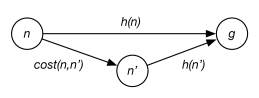
\includegraphics[scale=0.9]{disuguaglianzaTriangolare.png}
\caption{Disuguaglianza triangolare}
\end{center}
\end{figure}

La coerenza e la restrizione monotona possono essere intese in termini di disuguaglianza triangolare , che specifica che la lunghezza di qualsiasi lato di un triangolo non può essere maggiore della somma delle lunghezze degli altri due lati. In coerenza, il costo stimato per andare da n all'obiettivo non dovrebbe essere superiore al costo stimato per raggiungere prima n' e poi l'obiettivo. La funzione euristica della distanza euclidea (la distanza in linea retta in uno spazio euclideo multidimensionale) tra due punti quando la funzione di costo è distanza è coerente. Anche una funzione euristica che è una soluzione a un problema semplificato con soluzioni più brevi è in genere coerente.

\textbf{Proposizione}
\begin{center}
Con un'euristica consistente, la potatura multipla di percorso non può mai prevenire un ricerca A* dal trovare una soluzione ottima.
\end{center}

Quindi la ricerca A* include la potatura a più percorsi, s A* viene utilizzato senza potatura a più percorsi, la mancanza di potatura dovrebbe essere esplicitata. Spetta al progettista di una funzione euristica garantire che l'euristica sia coerente, in modo da trovare un percorso ottimale. L'eliminazione di più percorsi include l'eliminazione del ciclo, perché un ciclo è un altro percorso verso un nodo e pertanto viene eliminato. L'eliminazione di più percorsi può essere eseguita in tempo costante, impostando un bit su ciascun nodo a cui è stato trovato un percorso se il grafico è memorizzato in modo esplicito o utilizzando una funzione hash. La potatura a più percorsi è preferibile alla potatura a ciclo per i metodi in ampiezza in cui praticamente tutti i nodi considerati devono essere comunque archiviati. La ricerca in profondità non deve memorizzare tutti i nodi alla fine dei percorsi già espansi; la loro memorizzazione per implementare la potatura a più percorsi rende la ricerca in profondità esponenziale nello spazio. Per questo motivo, la potatura del ciclo è preferita alla potatura a più percorsi per la ricerca in profondità.

La potatura di più percorsi non è appropriata per IDA*, perché lo spazio richiesto per archiviare il set esplorato è in genere superiore allo spazio richiesto per A*, vanificando così lo scopo dell'approfondimento iterativo. È possibile utilizzare la potatura ad anello IDA*.

FARE QUESTA SEZIONE https://artint.info/2e/html/ArtInt2e.Ch3.S8.html
\end{document}



